
\documentclass [PhD] {uclathes}

% \input {mymacros}                         % personal LaTeX macros
\usepackage[round]{natbib}
\def\newblock{\ }
\usepackage[T1]{fontenc}
\usepackage{times}
\usepackage{latexsym}
\usepackage[utf8]{inputenc}
\usepackage{graphicx}
\usepackage{multirow}
\usepackage{microtype}
\usepackage{inconsolata}
\usepackage{subcaption}
\usepackage{amsfonts,amssymb}
\usepackage{booktabs}
\newlength{\wdth}
\newcommand{\strike}[1]{\settowidth{\wdth}{#1}\rlap{\rule[.5ex]{\wdth}{.4pt}}#1}
\newcommand{\sbN}{\scalebox{1.25}{$N$}}


%%%%%%%%%%%%%%%%%%%%%%%%%%%%%%%%%%%%%%%%%%%%%%%%%%%%%%%%%%%%%%%%%%%%%%
%
% Usually things live in separate flies.
%
% \input {prelim}                           % preliminary page info

%%%%%%%%%%%%%%%%%%%%%%%%%%%%%%%%%%%%%%%%%%%%%%%%%%%%%%%%%%%%%%%%%%%%%%%%
%                                                                      %
%                          PRELIMINARY PAGES                           %
%                                                                      %
%%%%%%%%%%%%%%%%%%%%%%%%%%%%%%%%%%%%%%%%%%%%%%%%%%%%%%%%%%%%%%%%%%%%%%%%

\title          {Mitigating Gender and Racial Bias \\
                in Automated English Speaking Assessment}
\author         {Alexander Kwako}
\department     {Education}
% Note:  degreeyear should be optional, but as of  5-Feb-96
% it seems required or you get a year of ``2''.   -johnh
\degreeyear     {2023}

%%%%%%%%%%%%%%%%%%%%%%%%%%%%%%%%%%%%%%%%%%%%%%%%%%%%%%%%%%%%%%%%%%%%%%%%

\chair          {Michael H. Seltzer}
\member         {Mark P. Hansen}
\member         {Li\ Cai}
\member         {Kai-Wei\ Chang}

%%%%%%%%%%%%%%%%%%%%%%%%%%%%%%%%%%%%%%%%%%%%%%%%%%%%%%%%%%%%%%%%%%%%%%%%

\dedication     {\textsl{To my partner, Kathryn, and my mom, Jamie, \\
                                  who deserve credit for at least 95\% of all my good fortune, \\
						  including having finished this dissertation, \\
						  and having been able to study with the incredible faculty at UCLA}}

%%%%%%%%%%%%%%%%%%%%%%%%%%%%%%%%%%%%%%%%%%%%%%%%%%%%%%%%%%%%%%%%%%%%%%%%

\acknowledgments {
I would like to express my deepest gratitude and appreciation to all those who have contributed to the completion of this dissertation. I extend my heartfelt thanks to my advisor, Mike Seltzer, for accepting me into the Social Research Methodology division, and for providing endless support, reassurance, and encouragement to follow my interests. And whose great taste in music has given me the chance to hear new jazz and rock music and musicians! I am truly grateful for his mentorship and constant encouragement throughout this journey.

My thanks go out to all the members of my dissertation committee. To Mark Hansen, for encouraging me to apply for the Transdisciplinary Research Acceleration Grant, for his belief in and guidance throughout this project, and for providing thoughtful and insightful feedback at every step of the way. To Li Cai, for always being available for a statistical consult, and for sharing the breadth of his expertise and wisdom about language assessment. To Kai-Wei Chang, for his commitment to sharing his knowledge of Natural Language Processing with others outside of the Computer Science department, for embarking on this interdisciplinary project, and for generously sharing his resources with us in Education. 

I would also like to extend my appreciation to John Rogers, for being a role model of what great leadership looks like, and for showing me how scholarship can make an impact in the world. And my thanks to Bill Sandoval, who introduced me to educational research, and who welcomed me onto his team in my most formative years at UCLA. 

My deepest gratitude goes out to my family and my partner. To my mom, for her commitment to my education, for her unconditional love and support, and for cultivating my intellectual curiosity and openness to new ideas. To my dad, for his calm support, and his veneration for serious thinking. To my brother, for teaching me the power of tenacity, for being a vigilant friend, and for renewing my interest in math and beyond. And of course to my partner, Kathryn, to whom I owe my present happiness, who taught me that I could love writing and thinking as an academic, whose curiosity and ways of thinking are an endless source of inspiration. 

To all those who have supported me that I have failed to mention, I offer my sincere appreciation. Your contributions, both big and small, have played a significant role in the completion of this dissertation. Thank you for being a part of this transformative experience. 
}



%%%%%%%%%%%%%%%%%%%%%%%%%%%%%%%%%%%%%%%%%%%%%%%%%%%%%%%%%%%%%%%%%%%%%%%%

\vitaitem   {2010}
                {B.A.~(Liberal Arts),
                St. John's College.}
\vitaitem   {2017}
                {M.A.~(Education), 
		UCLA.}
\vitaitem   {2016--2018}
                {Graduate Student Researcher, Developing Teachers' Capacity to Promote Argumentation in Secondary Science, UCLA.
                Collaborated with secondary school science teachers on implementing Next Generation Science Standards, with a focus on classroom discussion.}
\vitaitem   {2018--2022}
                {Graduate Student Researcher, Institute for Democracy, Education, and Access, UCLA.
                Analyzed national survey of U.S. public high school principals. 
		Prepared public-facing reports and articles for academic journals.}
\vitaitem   {2021--2022}
                {Graduate Student Researcher, Center for Research on Evaluation, Standards, and Student Testing, UCLA. 
		Contributed to university efforts to understand effects of COVID on undergraduate experience. 
		Refined survey to understand state-level approaches to English Language Learner pedagogy.}
\vitaitem   {2021--2022}
                {Researcher, Transdisciplinary Research Acceleration Grant, UCLA.
		Developed proposal to study the use of debiasing techniques in automated English speaking assesment.}
\vitaitem   {2022--2023}
                {Dissertation Year Fellowship, UCLA.
		For the study of measurement and mitigation of bias in automated English speaking assessment.}

%%%%%%%%%%%%%%%%%%%%%%%%%%%%%%%%%%%%%%%%%%%%%%%%%%%%%%%%%%%%%%%%%%%%%%%%

\publication    {\textsl{Patterns of classroom talk through participation in discourse-focused teacher professional development.}
	                Proceedings of the 13th Annual International Conference of the Learning Sciences, 2018}
\publication    {\textsl{What is this thing called a mechanism? Findings from a review of realist evaluations.}
                	New Directions for Evaluation, 2020.}
\publication    {\textsl{Do Adolescents Want More Autonomy? Testing Gender Differences in Autonomy Across STEM.}
	                Journal of Adolescence, 2021.}
\publication    {\textsl{Do Politics in Our Democracy Prevent Schooling for Our Democracy? Civic Education in Highly Partisan Times.}
	                Democracy \& Education, 2021.}
\publication    {\textsl{Using Item Response Theory to Measure Gender and Racial Bias of a BERT-based Automated English Speech Assessment System.}
                	Proceedings of the 17th Workshop on Innovative Use of NLP for Building Educational Applications, 2022.}
\publication    {\textsl{Principals’ Responses to Student Gun Violence Protests: Deter, Manage, or Educate for Democracy.}
                	Teacher’s College Record, 2023.}

%%%%%%%%%%%%%%%%%%%%%%%%%%%%%%%%%%%%%%%%%%%%%%%%%%%%%%%%%%%%%%%%%%%%%%%%

\abstract{
Automated assessment using Natural Language Processing (NLP) has the potential to make English speaking assessments more reliable, authentic, and accessible. Yet without careful examination, NLP may exacerbate social prejudices based on gender or native language (L1). Current NLP-based assessments are prone to such biases, yet research and documentation are scarce. Considering the high stakes nature of English speaking assessment, it is imperative that tests are fair for all examinees, regardless of gender or L1 background. This project addresses the need for studies in English speaking assessment through a series of three studies. In Study 1, I measure the accuracy of automated transcription, a key component of automated speaking assessments. In Study 2, I analyze a specific type of bias known as differential item functioning (DIF), and determine what patterns of DIF are present in human rater scores; moreover, I evaluate whether patterns of DIF are exacerbated by a pretrained, large language model (LLM) known as BERT. Lastly, in Study 3, I compare two approaches of mitigating DIF. Results from Study 1 indicate that there are indeed biases in automated transcription, however these do not translate into higher or lower scores. In Study 2, it is shown that BERT does (albeit to a small degree) exacerbate human rater biases. Finally, Study 3 demonstrates that it is possible to debias human and automated scores; however, the two approaches have serious limitations, particularly when the source of DIF is unknown. 
}

%%%%%%%%%%%%%%%%%%%%%%%%%%%%%%%%%%%%%%%%%%%%%%%%%%%%%%%%%%%%%%%%%%%%%%%%



\begin {document}
\makeintropages

%%%%%%%%%%%%%%%%%%%%%%%%%%%%%%%%%%%%%%%%%%%%%%%%%%%%%%%%%%%%%%%%%%%%%%
%
% Ordinarily each chapter (at least) is in a separate file.
%
%\input {chapter1}                         % Chapter 1 of dissertation
%\input {chapter2}                         % Chapter 2
%\input {chapter3}                         % etc.
%\input {chapter4}
%\input {chapter5}
%\input {chapter6}
%\input {chapter7}
%\input {chapter8}

\chapter{Introduction}

Automated assessment of non-native (L2) English speaking proficiency is made possible by recent advances in Natural Language Processing (NLP). Researchers have shown, for instance, that pretrained large language models (LLMs) can accurately replicate human rater scores in English speaking assessment \citep{wang2021automated}. Although applications of NLP present new opportunities for language assessment, recent studies have revealed that NLP can propagate and, in some cases, amplify negative stereotypes of marginalized groups \citep{blodgett2020}. Societal biases become embedded in NLP models, which may lead to unfair scoring, e.g., where examinees of a particular racial background are systematically given lower scores than others (Wang et al., 2018). Perhaps more commonly, biases of NLP-based assessments are not examined at all \citep[e.g.][]{collier2020test, ormerod2022automated}). 

Considering how widespread and high stakes English speaking assessments are at both the primary and secondary education levels \cite{cimpian2017, ets2005}, it is imperative that these assessments be fair for all students, regardless of gender or racial background. This dissertation presents a set of three studies aimed to address the need for deeper analyses of bias in automated assessment of non-native (L2) English speaking. 

This study draws on data from the English Language Proficiency Assessment for the Twenty-First Century (ELPA21), a collaborative of 7 state education agencies in the U.S. \citep{huang2018english}. Both the quantity and quality of data, as well as the consortium’s openness to research, make ELPA21 an ideal context in which to study biases of automated assessments.

In addition to examining gender and racial biases, I explore the use of debiasing techniques to mitigate such biases \citep{sun2019mitigating}. As debiasing is a relatively new area of research and has not yet been applied to language assessments, the primary goal is to examine advantages as well as disadvantages afforded by various approaches. This project addresses important gaps in English speaking assessment systems, so that NLP may be applied responsibility, in order to ensure fairness for all examinees.

\section{Automated speaking assessments}

English language assessment is mandated in the United States by the Every Student Succeeds Acts \citep{essa2015}. Tests are administered to over 4 million K-12 students annually \citep{irwin2021report} and, for university admissions, over 500,000 students take the Test of English as a Foreign Language \citep[TOEFL][]{ets2005}. Importantly, these test are often high stakes \citep{cimpian2017}.

In order to cut costs and meet the rising demand for English language assessments, some test developers have transitioned to fully automated assessment systems. These systems automate all aspects of English language assessment, including speech and writing, which in the past have been scored solely by human raters \citep{evanini2017approaches}. Several researchers, however, have questioned the fairness of automated speaking assessment systems, particularly for examinees of minority groups \citep{wang2018monitoring, collier2020test}.

\section{Advantages of automation}

While the advantages of NLP-based assessments are typically framed in terms of efficiency and affordability, NLP also has the capacity to improve reliability and even advance social justice-oriented goals. In the testing literature, it is well known that human raters are subject to cognitive and social biases \citep{engelhard2002monitoring}. Psychometricians often categorize these biases based on whether raters tend toward excessively severity or leniency, or whether they are prone to halo effects \citep{saal1980}. These biases persist even in the face of training and monitoring \citep{engelhard1994examining}, indicating that they operate at an unconscious level \citep{spencer2016}, which make them difficult to address.

Automated systems, in contrast to human raters, are not prone to the same kind of inconsistencies or unconscious bias. Indeed, automated scoring can promote fidelity of scores by identifying and mitigating human rater errors \citep{bejar2011validity}. \citet{wang2018monitoring} have demonstrated how automated systems can be used to identify overly lenient or harsh human raters in the TOEFL exam: A similar approach, though not yet attempted, could be used to identify raters with biases against minoritized groups.

While not prone to the same sorts of errors as human raters, automated systems can still be biased. However, there are methods for identifying and mitigating such biases in NLP-based applications. \citet{zhao2018gender}, for example, have shown how it is possible to debias an NLP-based application that resolves coreferences (e.g., identifying subjects of sentences when pronouns are ambiguous). Originally, the application was more likely to ascribe historically male professions (such as politician or doctor) to male subjects; however, after supplementing the corpus with less biased data, the model became more gender-neutral in its coreference resolutions. Whether social biases are present in humans or in automated systems, they can be measured and mitigated with careful planning and engineering.

\section{Examples of bias and debiasing}

There is little research on bias in automated testing of English speaking proficiency. In order to illustrate what sorts of problems might occur with these systems, I consider two hypothetical examples of how biases might become embedded in automated English language assessment systems, and how bias reduction techniques could be used to address them.

\subsection{Insufficient training data for automated speech recognition}

Automated speech recognition (ASR) systems have been shown to be less accurate for non-White speakers \citep{koenecke2020} and, in some cases, less accurate for women \citep{tatman2017a, tatman2017b}. These disparities may be due to lack of representation in the data itself \citep[e.g.][]{zhao2018gender}. In English language assessment, a less accurate ASR system will generate less accurate transcripts, which equates to less accurate scores for language-minority examinees. Beyond transcription accuracy, when ASR systems are also used to generate linguistic features (e.g., pronunciation scores), language-minority examinees may be given lower scores.

One possible debiasing solution for language assessment systems that lack sufficient data for language-minority groups is to implement a filtering model. The filtering model could flag some responses as non-scorable and send them to human raters for review. Bypassing automated scoring in some cases may help to ensure that certain examinees (e.g., who are known to have less accurate transcripts) are not penalized by the ASR system.

A more comprehensive solution would be to use a technique known as data augmentation \citep[e.g.][]{zhao2018gender}. A simple version of data augmentation is simply to duplicate the data of underrepresented groups to artificially make them more representative. Although requiring more effort, it is also possible to apply various transformations to audio data (e.g., changing the pitch of male and female respondents, or mixing and matching speakers with different accents). These transformations would help to prevent the model from learning construct-irrelevant features like pitch or accent. This approach would remove the ability of the model to learn differences in race or gender at the data-level.

\subsection{Implicit bias in human ratings}

Scholarship on implicit bias demonstrates that human behavior is influenced unconsciously and in diverse contexts by culturally-embedded associations \citep{greenwald2006implicit}. These associations, including negative stereotypes about underrepresented groups, typically operate independently of individuals’ explicit attitudes \citep{karpinski2001attitudes} and they are often activated by peripheral cues \citep{spencer2016}.

In the context of English speaking proficiency, it is possible that examinees’ accents may trigger human raters’ implicit biases. For instance, as a whole, the U.S. population has an implicit bias against faces that have Arabic features \citep{park2007implicit}; it is possible that hearing a Middle Eastern accent might prompt a rater from the U.S. to (unwittingly) give a lower score. Based on research on the salience of peripheral cues, such bias would be more likely to be present when raters hear adult voices with heavier accents, and for raters who are distracted, hungry, or otherwise on autopilot.

In addition to filtering and data augmentation, another technique that would ameliorate the propagation of implicit bias is retraining the model using adversarial neural networks. Widely applicable to a number of problems encountered in deep learning, adversarial networks actively prevent the model from learning certain information. Following the example of \citet{zhang2018mitigating}, it would be possible to ensure that the language model is unable to predict the ethnic origin of examinees’ responses. In removing its ability to infer race or gender, it may also remove the source of implicit bias.

\section{Overview of study design}

The general research design involves four main components: using automated transcription services to generate text from speech, constructing a language model to score examinees’ (transcribed) text, measuring gender and racial bias via analysis of differential item functioning (DIF), and exploring solutions for debiasing models. Speaking items were selected from the English Language Proficiency Assessment for the 21st Century (ELPA21), to reflect a range of ages and expected duration of response. It is hypothesized that adult voices and longer items will trigger more implicit bias, and hence will be more likely to show DIF. As a part of this analysis, I also examine biases in the automated speech recognition (ASR) system by calculating word error rate (WER) of speech-to-text transcripts. 

In this study of racial and gender bias, I focus on a specific type of bias known as differential item functioning (DIF), common in educational and psychological assessment \citep{aera2014}. Briefly, DIF occurs when equally proficient individuals who belong to different groups (e.g., male and female) are given consistently different (i.e., higher or lower) scores for certain items. Although items in all large-scale assessments have been analyzed for DIF, including ELPA21 \citep{anderson2015elpa21}, there are multiple methods of testing for DIF, and patterns of DIF may change over time (e.g. since the initial development of the test). The specific approach that I use to identify DIF is specifically suited to the context of this research study.

Debiasing NLP-based applications is a relatively new field of research. It will be of interest to compare multiple methods of debiasing, and to determine how well each addresses DIF.

These research goals are organized in three interconnected studies: 

\begin{enumerate}
    \item In Study 1, I quantify the biases of large-scale, automated transcription services, by comparing average WER, disaggregated by gender and L1 background.
    \item In Study 2, I examine DIF in human raters and an LLM-based automated scoring system, to see if the LLM-based automated scoring system introduces or exacerbates any patterns of DIF. 
    \item In the third study, I explore two techniques to mitigate bias in automated systems, each with their own advantages and limitations.
\end{enumerate}

The specific research questions that each study addresses are enumerated in the respective chapters. Since they share a common aim, however, they also draw from the same source of relevant literature and methods, which will be discussed altogether.



\chapter{Literature Review}

This study is situated at the intersection of (1) English speaking assessment, (2) measurement of bias, and (3) language modeling. With respect to English speaking assessment, I review (a) relevant literature on the prevalence and high stakes nature of English speaking assessment in the United States, and (b) automated speaking assessment systems currently in use. With respect to measurement of bias, I discuss (a) the impact of gender and L1 on L2 English speaking proficiency, and (b) differential item functioning (DIF) both in general and as it relates to English speaking assessment. Finally, with respect to language modeling, I review research on large language models (LLMs), how these models become embedded with societal biases, and how some researchers have been able to debias LLMs. 

\section{English speaking assessment}

\subsection{English speaking assessment in the United States}

English language assessment is widespread and often holds high stakes for examinees in the United States. The Every Student Succeeds Acts \citep{essa2015} requires states to administer English language assessments to all students from non-English speaking homes, and tests are administered to over 4 million K-12 students annually \citep{irwin2021report}. English language assessments are also prevalent at the post-secondary level: Every year, over 500,000 examinees take the Test of English as a Foreign Language (TOEFL), administered by Educational Testing Service \citep{ets2005}, and 3.5 million people take the International English Language Testing System \citep{ielts2023}. In terms of real-world impact, many universities require applicants to score above a certain threshold of proficiency on the TOEFL or IELTS as an admission requirement. For K-12 students, being classified as an “English learner” decreases high school graduation rates and college-going behavior \citep{johnson2019effects}.

Nearly all language assessments include speaking as one of four language proficiency domains, along with listening, reading, and writing \citep{ccsso2012framework}. At the K-12 level, speaking tasks are usually open-ended, yet have a narrow contextual focus; for instance, students are asked (via written or verbal prompt) to describe what is happening in a picture \citep{luoma2004assessing}, At the post-secondary level, examinees are given more challenging tasks, e.g., talking about a particular topic for several minutes. For most assessments, examinees speak into a microphone and responses are scored by a human rater or an automated system. Using a slightly different approach, \citet{ielts2023} employees trained interviewers to administer and score speaking proficiency in a face-to-face setting.

For K-12 students, the majority of states administer assessments developed by one of two consortia, World-Class Instructional Design and Assessment (WIDA) or English Language Proficiency Assessment for the 21st Century (ELPA21). Neither consortium currently uses automated speaking assessment: Rather, for speaking items, test-takers speak into a microphone for 5-10 seconds, whereafter their responses passed along to human raters to score.

There are two states, however, that do use automated assessment for K-12 speaking proficiency. Both states use systems developed and administered by Pearson. The Texas English Language Proficiency Assessment System (TELPAS) uses Versant, one of the first automated speaking proficiency assessments, originally developed for large businesses and administered over the telephone \citep{pearson2019versant}. Given the lack of validity studies and potential unreliability of its automated system, TELPAS’ recent switch to Versant has sparked some skepticism among academics \citep{collier2020test}. Pearson also helped to develop the speaking assessment for the Arizona English Language Learner Assessment (AZELLA), seemingly independent of Versant \citep{johnston2019using}. At the post-secondary level, TOEFL uses an automated speaking assessment system known as SpeechRater, developed by researchers at ETS \citep{chen2018automated}.

\subsection{Current NLP-based automated speaking assessments}

\citet{chen2018automated} identify four primary components of automated speaking assessment systems: (1) an automated speech recognition (ASR) system, which includes speech-to-text transcription, (2) the extraction of linguistic features from audio and text data, (3) a filter model to identify non-scorable responses (e.g., those with audio errors or potential plagiary), and (4) a scoring model to combine linguistic features into a single score.

Depending on the purpose or sophistication of the automated assessment system, some of the above steps may be combined or omitted. Pearson, for instance, appears to omit the filter model (step 3) for TELPAS and AZELLA. In a different vein, \citet{chen2018end} have experimented with combining steps 1, 2, and 4 into a single end-to-end model. (Models are described as end-to-end when multiple intermediate processes get subsumed within a single architecture.) Although the performance of end-to-end models can be impressive, they are a black box—that is, the linguistic features that the model learns and uses to score examinees’ responses are hidden. For this reason, it can be challenging to interpret or debug end-to-end models.

\subsubsection{(1) Automated speech recognition}

The ASR system built by ETS is comprised of multiple parts, and used for multiple purposes. Under the hood, it uses a Hidden Markov Model to parse phonemes (i.e. syllables), an n-gram model to track word dependencies, and a weighted finite state transducer to limit the search space \citep{qian2019automatic}. Combined, these three components are able to generate transcripts and assign probabilities to text. The transcripts are used for further data processing, while the probabilities associated with the transcripts may be used as a linguistic feature (referred to as the “Average ASR Confidence Score”) in the scoring model \citep{zhang2019assessing}.

Training ASR systems requires a prolific amount of labeled data (i.e., audio files accompanied by accurate transcripts). The exact amount of training data required to build an ASR system depends on the complexity of the speech. For speech assessment purposes, \citet{qian2019automatic} suggests on the order of a million words; \citet{evanini2017approaches} suggests 200-300 hours of speech. Data can be supplemented with external speech corpora, e.g., the Switchboard corpus \citep{godfrey1997switchboard}, in order to improve the accuracy of speech-to-text transcription; but ensuring recording quality across data sources can be challenging \citep{qian2019automatic}.

Even with external data, there may yet remain a significant amount of transcription error. A common index of transcription accuracy is word error rate (WER), which is the ratio of the total number of errors (i.e. erroneous insertions, deletions, or substitutions) to the total number of words in a given transcript or corpus \citep{qian2019automatic}. (See Section \ref{methods_wer} for details regarding how WER is computed.) Human-human transcription of non-native speech typically yields a WER of 15-20\% \citep{zechner2009}. SpeechRater comes close to human parity, with a WER of 23\% for non-native spontaneous speech \citep{tao2016exploring}. AZELLA has a higher WER of 35\% \citep{cheng2014automatic}. By contrast, human-human WER of native speech cam be as low as 5\% \citep{xiong2016achieving}.

One of the significant challenges of transcribing non-native speech is faithfully capturing errors. Rather than reproduce errors, ASR systems tend to predict a similar (grammatically correct) phrase. One internal study showed that SpeechRater failed to capture 70\% of non-native speakers’ grammatical errors \citep{yoon2019features}.

\subsubsection{(2) Linguistic features}

Once audio data has been transcribed, linguistically-relevant features are extracted from text and audio data. Linguistic features are typically defined a priori, in alignment with standards of speaking proficiency \citep[e.g.][]{brown2005examination}. For instance, to assess fluency, SpeechRater calculates (among other things) the number of pauses, the duration of pauses, and the number of words per second in examinees’ speech \citep{hsieh2019features}. To assess vocabulary, SpeechRater calculates the number of unique words that examinees use \citep{yoon2019features}. In TOEFL, over 60 linguistic features have been examined as candidates for speech assessment. (Note: In an end-to-end model, these a-priori decisions about which linguistic features to use are not possible, since the features are latent.)

\subsubsection{(3) Filter model}

A filter model helps to reduce error in the automated system by identifying “non-scorable responses” \citep{loukina2019scoring}. Such responses may have had audio issues; alternatively, they may be the result of uncooperative examinees or plagiary. In such cases, examinees’ responses may bypass the automated assessment system, and instead be designated for human rating. Common technical difficulties include the presence of background noise and mechanical issues with recording devices; as described above, ASR systems can be sensitive to slight discrepancies in audio quality, which may produce inaccurate transcripts and, subsequently, inaccurate test scores. There are also instances in which a filter model can be used to identify examinees who are cheating or otherwise gaming the system.

The filter model is helpful in improving the ASR system by acting as a manual override. Automated assessment systems are known to have certain weaknesses, and rather than build a system that is capable of handling every type of exception, it may be more cost-effective to bypass the automated assessment system in certain cases.

\subsubsection{(4) Scoring model}

The scoring model combines linguistic features to produce a summative language proficiency score for examinees \citep{loukina2019scoring}. Finding an appropriate scoring model also requires a lot of data. In order to train a scoring model for complex constructed item types, \citet{zechner2019summary} suggests having at least 10,000-20,000 pre-scored responses. More complicated scoring models, however, might require significantly more data.

TOEFL uses linear regression, wherein features are weighted and selected using a LASSO-based method \citep{loukina2015feature}. The primary rationale for using linear regression is that it is relatively transparent and easy to communicate; \citet{loukina2019scoring} report that ETS has experimented with more complex scoring models, e.g., random forests, but they were not worth the 2-3\% improvement in accuracy. \citet{zechner2019summary} reports that, at the item-level, their scoring model is more reliable than human-human reliability coefficients ($r$ = 0.65, compared to $r$ = 0.55-0.60). In contrast to TOEFL, AZELLA combines features using a deep learning model with a single layer of latent variables \citep{cheng2014automatic}.

\section{Bias in English speaking assessments}

\subsection{Issues of fairness in automated speaking assessment}

During the course of test development, it is standard practice for a bias review committee to screen all items for inappropriate or content-irrelevant material, and to analyze items for differential item functioning (DIF) to ensure quantitatively that items are not biased against any particularly groups of examinees, e.g., women or racial minorities \citep{aera2014}. It is likely that DIF analyses were conducted by Pearson and ETS for speaking items scored by human ratings, but it is not clear whether they were repeated for automated scoring systems. Given that Versant (Pearson’s ASR system for TELPAS) was not originally designed to assess K-12 students, and some evidence of inconsistency among examinees’ scores \citep{collier2020test}, it is troubling such analyses have not been made public (or, possibly, even conducted).

\subsection{Impact of gender and L1}

Most of the research on the impact of gender and L1 on language proficiency touches on myriad aspects of language proficiency, and is not specific to speaking proficiency. In general, female examinees perform better than male examinees on language assessments \citep{reilly2019gender}, and this typically including L2 English language assessments \citep{denies2022mapping}. These differences have early developmental roots, e.g., in word acquisition \citep{kaushanskaya2013gender} and phonetic acquisition \citep{dodd2003phonological}. Importantly, gender differences vary by socio-cultural factors \citep{denies2022mapping}, and others have pointed out that some language tasks do seem to favor males \citep{wucherer2018language}. 

Native language (L1) also impacts L2 English speaking proficiency. The literature on "language transfer" or "cross-linguistic influence" focuses on similarities and differences between language structures \citep[][p. 257]{brown2000principles}. One intuitive finding, for instance, states that examinees perform better on vocabulary tests when there are more L1 cognates \citep{lesniewska2018first}. Other literature examines the complex socio-cultural factors that play a role in the development of L2 English speaking. For instance, \citet{derwing2013development} attribute differences between Slavic and Mandarin English speaking proficiency to factors like age, motivation, and conversational opportunities, which interact with L1 in complex ways. 

\subsection{Differential item functioning}
\label{intro_dif}

This study focuses on a specific type of bias in English speaking proficiency known as differential item functioning (DIF). Historically, interest in DIF grew out of a movement in the 1960s to make standardized assessments more fair for racially underrepresented minorities by removing cultural bias from test items \citep{angoff1993}. Approaches to identifying DIF continue to be used in test development to screen items for potential bias against specific groups. For example, an item with extensive references to the Bible would give Christian examinees an advantage. Such references would not be appropriate unless the explicit goal of the test was to measure knowledge of Christian theology, otherwise the item would be measuring a content-irrelevant construct \citep{aera2014}.

In educational assessment, a test item is said to exhibit differential item functioning (DIF) when “equally able (or proficient) individuals, from different groups, do not have equal probabilities of answering the item correctly” \citep[][p. 4]{angoff1993}. By definition, DIF is not a measure of first-order group differences (or mean group differences), which is sometimes referred to as impact. Rather, DIF conditions on overall (and ideally unbiased) proficiency. In other words, DIF occurs when examinees who should receive similar scores (based on their performance on other test items) receive different scores on a specific item under review. In DIF terminology, overall proficiency is referred to as the matching criterion, the majority group is referred to as the reference group and the minority group is referred to as the focal group.

For instance, in college admissions tests of reading comprehension, males (the reference group) tend to score higher on science-related passages, whereas females (the focal group) tend to score higher on humanities-related passages, conditional on examinees’ overall language proficiency \citep[the matching criterion;][]{steedle2023}. 

There are many possible causes of DIF. The above example highlights the possibility of confounding variables \citep[e.g. males tend to major in STEM at a higher rate;][]{sloane2021college}. One of the central concerns of this paper is that DIF might arise from implicit bias in human raters—that is, human raters might be unconsciously influenced by phonic features in examinees’ voices. Also pertinent to this study, DIF could be caused by discrepancies in automated transcription of speech, or socio-cultural or cognitive differences rooted in examinees’ gender or L1 backgrounds. Practitioners have lamented that determining causes of DIF is challenging and often yield inconclusive results \citep{zumbo2007}. 

\subsubsection{DIF based on gender and L1}

Although there are many studies of DIF with respect to gender and L1 in large-scale English language assessment, most of these studies focus on vocabulary, listening, and writing proficiency \citep{kunnan2017evaluating}. There are very few studies that focus on English speaking proficiency. 

Although DIF analyses of automated speaking assessment systems are not publicly available. \citet{wang2018monitoring} have conducted some analyses of bias in SpeechRater. Analyzing examinees’ overall scores, they found SpeechRater to be somewhat partial towards some groups over others, based on examinees’ native language. Although they suggested some plausible explanations for these discrepancies, e.g., an overall "[reduced number] of predicted scores at the extremes of the scoring scale" (p. 117), they concluded that more research was needed to explore these hypotheses.

\subsubsection{Sources of DIF}

Issues of fairness in automated speaking assessment are underexplored (or underreported), but examinations of sources of bias are practically non-existent. Based on literature in adjacent fields, however, it is possible to construct a list of likely sources of bias in automated speaking assessment. 

\noindent \textbf{Automated transcription bias} \;

One potential source of bias in automated speaking assessment is automated transcription. \citet{dichristofano2023} has shown that the largest providers of automated transcription services (Google, Amazon, and Microsoft) all have discrepancies in transcription accuracy based on speakers’ native language (L1) background. As text transcripts constitute the most important (and sometimes exclusive) input for most NLP-based scoring systems, it is important to consider these discrepancies, as they may lead to discrepancies in scores.

\noindent \textbf{Human rater bias} \;

Another potential source of DIF lies in the quality of human ratings. Although human ratings are often considered the gold standard, and the benchmark against which to evaluate the success of automated scoring systems \citep{zhang2019assessing}, human ratings are not ideal scores. An ideal score would be "assigned by a panel of [unbiased] expert raters and represent the true score of a spoken response" \citep{zechner2019summary}. Although human raters receive training and are monitored over time to improve consistency \citep{engelhard2002monitoring}, human-human interrater reliability typically ranges between 0.55 and 0.60 on individual items \citep{zechner2019summary}. 

Scholarship on implicit bias demonstrates that human judgment is influenced unconsciously by peripheral cues, including speakers’ accents \citep{kang2021social}. These biases may lead to unfair scoring without raters even realizing it \citep{greenwald1995}. Indeed, \citet{winke2013} reports that human raters are more lenient towards examinees who share the same L1 background. In a summary of research on the biases of raters of L2 English, \citet{lindemann2013reliably} reports a strong disconnect between subjective evaluation of speech (e.g. using Likert scales) and more objective measures (e.g. transcription). One limitation with these studies is that they assume that L2 English speakers are of similar proficiency levels, and it is not clear whether the researchers controlled for speakers’ English proficiency. 

Research on implicit bias and speech suggests that, in the context of English language assessment, there may be more bias in the domain of Speaking (e.g. as opposed to Writing). By listening to examinees’ voices, human raters may be more likely to be influenced by examinees’ accents, triggering implicit bias that affects their judgment during scoring.

\noindent \textbf{Sociocultural factors} \;

There are many socio-cultural differences based on gender and L1 that affect English speaking assessment. \citet{derwing2013development}, for instance, discuss how factors like age and conversational opportunities interact with L1 in complex ways. Gender is also a source of variation in L2 English speaking proficiency, although it varies by culture and task \citep{denies2022mapping}. 

There may also be cultural differences that interact with item properties. Now a classic example, \citet{freedle2003correcting} describes how verbal items draw on cultural knowledge that disadvantage minority examinees. It is possible that certain speaking items may require an understanding of the context of schooling in the U.S.; students of some racial backgrounds may be more familiar with these practices than others. 

\noindent \textbf{Feature bias} \;

One potential source of bias lies in the linguistic features and how they are combined in the scoring model. Although research has not yet examined this issue, \citet{zhang2019assessing} warns that "interactions of [features] and demographic groups can lead to subgroup biases" (p. 52). In broader terms, English speaking is not a monolithic construct, and without specifying these differences in the scoring model, speakers of some language-minority backgrounds might be unfairly downgraded. For instance, speakers of some ethnic backgrounds might enunciate more slowly which may not be a marker of proficiency but simply a regional difference. Failing to specify this in the model would lead to biased scores for these examinees.

The above problem illustrates how test fairness is impacted by design decisions. Indeed, it illustrates that there is a tradeoff between transparency and complexity. Researchers at ETS chose to make their system transparent by engineering many low-inference linguistic features that are combined via linear regression. This approach was chosen because it is a less “cumbersome representation” of speaking proficiency \citep[][p. 83]{loukina2019scoring}. Yet, speaking proficiency is not a simple construct. It may require non-linear combinations of multiple layers of latent variables to capture the complexity of fluency or discourse coherence. Choosing a more complex model, however, reduces the transparency of the linguistic features, and may make it more difficult to explore sources of bias.

\noindent \textbf{Machine learning bias} \;

NLP-based automated assessments often rely on machine learning methods, which are susceptible to introducing and exacerbating biases at multiple stages of development \citep{suresh2021framework}. Pretrained LLMs are especially susceptible to biases because they are trained on large corpora of text scraped from the web and social media \citep{blodgett2020}. Social biases in source text resurface in downstream applications, including machine translation \citep{stanovsky2019evaluating} and sentiment analysis \citep{kiritchenko2018examining}. In educational assessment, machine learning biases ultimately may influence examinees’ scores. 

In section \ref{lit_ml_bias}, I consider in greater detail how these sources of machine learning bias can occur in language modeling and in LLMs more broadly. 

\noindent \textbf{Other biases} \;

Although there are too many potential sources of DIF to review in full, I highlight several miscellaneous sources of DIF that bear on the inquiry of L2 English speaking assessment. \citet{huang2016exploring} report that curricula vary across countries, and that these differences are a likely source of DIF in international assessment. This source of bias would be related to the age at which examinees emigrated and entered into the U.S. schooling system. In another vein, it has been suggested that easier items might be more likely to exhibit DIF \citep{santelices2010unfair}, and guessing behavior, which is related to overall proficiency, may also be a source of DIF \citep{dorans2004examining}. Given that speaking is a difficult aspect of L2 language acquisition \citep{brown2000principles}, it is possible that examinees who are less fluent are able to guess their way through non-speaking items, but struggle with speaking items.

\section{Language modeling}

\subsection{Large language models}

Language modeling refers to the construction and use of probabilistic models for language generation and inferential tasks \citep{jurafskyspeech}. In automated language proficiency assessment, language modeling is used in multiple ways and at multiple stages of the automated assessment process. As described above, ETS uses multiple language models which, when combined, produce speech-to-text transcriptions and linguistic features relevant to speech proficiency \citep{qian2019automatic}.

Language models with at least 1 layer of variables between the input and the output are classified as deep learning models \citep{goodfellow2016deep}. Such models are often characterized as black boxes because the features that become embedded in the coefficients of the models are latent, and often unclear \citep[e.g.][]{gretter2019automatic}. Despite the inscrutability of deep learning models, they are popular because they are easy to deploy, adaptable to a variety of tasks, and often quite powerful. Although they are not widely used in language assessment, initial trials have shown that deep learning models are moderately more accurate than the more common approach of combining manually-constructed features \citep{chen2018end}.

A prolific amount of data is required to train most language models and, as a general rule, the more complicated the model, the more data is required. Currently there is on the order of 105 hours of speaking data publicly available \citep{galvez2021people}, and hundreds of terabytes of uncompressed text data \citep{iderhoff2023}. Industry leaders like Google and AWS, however, draw from considerably more data. Sophisticated language models, whether speech or text-based, take a lot of computational resources to train. RoBERTa, for instance, a text-based language model, is comprised of 108 parameters and was trained for five days on 1,024 × Nvidia 32GB V100 GPUs \citep{liu2019roberta}.

Because of the considerable costs involved in training language models, it is common to use a general language model as a foundation, and fine-tune the model (which requires significantly less data) to perform specific tasks; this technique is known as transfer learning \citep{jurafskyspeech}. With transfer learning, the theory is that the general language model can learn the complex semantic and grammatical dependencies of language by training on a large corpus of data. Using this general language model as a foundation, one can then train the model to perform various tasks using a much smaller dataset (sometimes only thousands of observations), and for a fraction of the computational resources (e.g., 1-2 GPUs for 8 hours).

One of the most widely used text-based general language models is Bidirectional Encoder Representations from Transformers (BERT), developed by \citet{devlin2018}. BERT was trained as a masked language model, which means it learned language by trying to guess the words in a sentence. More specifically, the model was presented with a sentence in which 15\% of the words are masked, and it must predict what those correct words are. The model is constructed such that it is able to learn dependencies between the masked word(s) and every other word in the sentence using an attention mechanism. Having trained the general language model, it is then fine-tuned to do a variety of tasks.

The performance of general language models, including BERT, are evaluated by their accuracy on various language tasks. One of the most widely used benchmarks is the 9 General Language Understanding Evaluation (GLUE) tasks \citep{wang2018glue}. GLUE tasks vary from identifying grammatically (in)correct sentences to assessing the (positive or negative) sentiment of movie reviews. BERT performs as well as humans on a number of these tasks.

\subsection{Bias in large language models}
\label{lit_ml_bias}

There is now a large literature on bias in artificial intelligence (AI), and bias in NLP more specifically. One branch of research has focused on classifying the types of socio-economic harms caused by biased AI \citep[e.g.][]{blodgett2020}. Because I have discussed the harms caused by biased automated assessment elsewhere, I focus instead on the technical aspects of how bias may be introduced to AI systems. \citet{suresh2021framework} outline seven steps in the AI pipeline in which bias may be introduced. The three sources of bias most pertinent to this study include (1) a type of representation bias, (2) a type of measurement bias, and (3) learning bias. I consider each of these sources of bias in greater detail below.

Although representation bias usually refers to a mismatch between the sample and the population, there are other types of representation bias. For instance, even if the sample is representative of the population, the population itself may contain subgroups too small for the model to learn. In other words, for certain small groups, there may not be enough data for the algorithm to learn how to make accurate predictions. Along these lines, it has been shown that ASR systems are less accurate for non-White speakers \citep{koenecke2020} and, in some cases for women \citep{tatman2017a, tatman2017b}. In the context of English language assessment, this may be a problem for examinees from language-minority backgrounds.

Part of the reason why representation bias is so prevalent in applications of AI is that deep learning models require a prodigious amount of data. Supplementing data with external speech corpora, e.g., Switchboard corpus \citep{godfrey1997switchboard}, improves the accuracy of speech-to-text transcription \citep{qian2019automatic}. Yet these external corpora may not be sufficiently large, especially for non-native speakers from minority-language backgrounds.

Measurement bias refers to systematic differences in the operationalization(s) of constructs. With respect to English speaking proficiency, measurement bias may occur when human raters consistently give lower (or less accurate) scores to individuals from a certain group. As discussed above, this may be caused by implicit biases \citep{spencer2016} or by interactions between linguistic features and demographic characteristics \citep{zhang2019assessing}. Because NLP-based assessments are trained on human-rated data, human biases may become embedded in the model(s).

Finally, learning bias results when specifications of the model itself are susceptible to introducing or exacerbating biases. As an example, \citet{suresh2021framework} mention how pruning, a common technique in large-scale AI models, often reduces prediction accuracy for small subgroups \citep{hooker2020characterising}. Such model design choices may also exacerbate existing biases. In one example, \citet{zhao2017men} found that their model predicted the gender of people in an image by their proximity to objects in the surrounding environment (e.g. women around kitchen appliances, men around computers) at approximately twice the frequency as was found in the original training data. Likewise, for speaking assessment, certain models may be less accurate for smaller groups, or they may amplify biases by fixating on certain acoustic or textual features (e.g., different accents).

One of the principal drawbacks of deep learning models is their inscrutability, and the difficulty of characterizing which features (or which biases) are learned by the model. Although ETS' SpeechRater relies primarily on manually-constructed features, one of their most predictive features, "Average ASR Confidence," is the output of deep learning models \citep{qian2019automatic}. Pearson does not share details of their models in technical documentation, but they do seem to employ a scoring model that uses deep learning \citep{cheng2014automatic}.

In addition to the above issues, general language models come prepackaged with their own set of biases that exist even prior to fine-tuning for specific speech tasks. These biases arise from the fact that general language models are pretrained on text from Wikipedia, online news outlets, and even community forums like Reddit \citep{liu2019roberta}. Given the biases that exist in these spaces, it is not surprising that applications of general language models often reflect strong cultural biases against women and people of color. For example, in coreference resolution, NLP models will associate historically male occupations (such as physician or politician) to masculine pronouns, and historical female occupations to female pronouns \citep{zhao2018gender}.

\subsection{Debiasing techniques}

There are several techniques that have been proposed for mitigating biases in NLP applications. \citet{sun2019mitigating} classify these techniques into two broad classes of methods, retraining and inference, based on the stage at which bias is addressed. In retraining, the goal is to train (or retrain) the model on an unbiased dataset or to change the way in which the model learns from data. Retraining reshapes the model at a more fundamental level, but it can also be more cumbersome or infeasible in practice. In contrast, inference-based methods address problems of bias further down the pipeline by constraining or rebalancing the models’ inferences or predictions. Retraining and inference methods are not mutually exclusive, yet researchers have not explored how they might be used in conjunction.

One comprehensive yet laborious retraining solution is known as data augmentation \citep[e.g.][]{zhao2018gender}. A simple way to augment data is to duplicate the data of underrepresented groups to artificially make them more representative, forcing the model to train on equal amounts of data from each group. A more elaborate approach for augmenting data might be to change the pitch of voices, so that male responses are made to occur in traditionally female registers, and vice versa. It would also be possible to mix accents by cutting and pasting responses from different examinees. This approach removes the ability of the model to learn differences in the pitch or accent of the speaker at the data-level, and may force it to focus on more relevant aspects of speech.

Another retraining technique employs adversarial neural networks. Widely applicable to a number of problems encountered in deep learning, adversarial networks actively prevent the model from learning certain information. Following the example of \citet{zhang2018mitigating}, an adversarial network would penalize the model (during training) for predicting the gender or ethnic origin of examinees’ responses. In removing its ability to infer race or gender, it may simultaneously remove the source of implicit bias. One of the benefits of adversarial neural networks is that mitigating bias may not require identifying the problematic features that the deep learning model has learned.

An example of an inference-based debiasing technique that may be relevant to the current project is constraining predictions. In the context of English language assessment, this may involve conditioning on overall language proficiency. That is, if we know that a group of language-minority examinees is equally proficient as the reference group (based on their performance on other test items), we could constrain the algorithm to give the focal group the same distribution of scores as the reference group on each speaking item. While this approach introduces additional dependencies, it may make the algorithm fairer in its treatment of examinees who face systematic bias.



\chapter{Methods}

\section{Data}

\subsection{ELPA21}

This study draws on data from the English Language Proficiency Assessment for the 21st Century (ELPA21), a consortium involving 7 state education agencies in the U.S. \citep{huang2018english}. Approval for this research project was granted by the ELPA21 consortium and the university institutional review board. To maintain confidentiality, certain details regarding test items and examinees are omitted. 

In most frameworks for English language assessment, Speaking is one of four language proficiency domains, along with Listening, Reading, and Writing \citep{ccsso2012framework}. At the K-12 level, speaking tasks are open-ended, yet have a narrow contextual focus; for instance, students are asked (via written or verbal prompt) to describe what is happening in a picture \citep{luoma2004assessing}. Examinees speak into a microphone for up to two minutes, after which their responses are passed along to human raters for scoring. All verbal responses in ELPA21 are currently scored by human raters. Human raters assign holistic integer scores based on scoring rubrics that vary by scale and item type. Consistent with best practices, human raters are trained and monitored over time to ensure consistency \citep{engelhard2002monitoring}. 

Analyses focused on two grade bands (2–3 and 9–12) which corresponded to two tests. Tests were administered during the 2020–2021 school year. Because different tests were developed for each grade band, we sampled examinees and selected test items to help ensure that these two sets of analyses were as comparable as possible. 

\subsection{Sample design and demographics}
\label{sec:meth_sample}

The sampling frame included all examinees in grade bands in 2–3 or 9–12 who met the following inclusion criteria: answered all three speaking items analyzed in this study; answered enough items in each of the other three sections to receive domain-specific scores; had gender and L1 demographic information available. Furthermore, to limit the scope of the study, we excluded examinees who had an IEP or 504 Plan, examinees with non-binary gender, and examinees whose L1 was not one of the ten L1s analyzed in this study. 

From the sampling frame, we sampled 15,000 students (8,377 from grade band 2–3, and 6,623 from grade band 9–12). The size of our sample was limited, in part, by the cost of automated transcription. We included all examinees whose L1 was one of our nine L1 focal groups (Table \ref{smp_dscr}). The remainder of examinees were randomly sampled from Spanish speakers. 

\begin{table*}[htbp]
\centering
\caption{\label{smp_dscr} \raggedright Sample descriptive statistics, in aggregate and disaggregated by gender and L1.}
% \small  % comment out this line if wanted bigger font size
\begin{tabular}{lccccccc}
\toprule
    & \multicolumn{3}{c}{\textbf{Grade Band 2-3}} & \multicolumn{1}{c}{ } & \multicolumn{3}{c}{\textbf{Grade Band 9-12}} \\
    \cline{2-4}
    \cline{6-8}
     & \textbf{n} & \textbf{\%} & \textbf{Avg. Proficiency} & & \textbf{n} & \textbf{\%} & \textbf{Avg. Proficiency} \\
    \midrule
    \textbf{All} & 8377 & 100 & 0.18 (0.91) & & 6623 & 100 & 0.16 (0.93) \\
    \textbf{Gender} &  &  &  & &  &  &  \\
    \hspace{3mm} Male & 4310 & 51.5 & 0.13 (0.9) & & 3648 & 55.1 & 0.14 (0.94) \\
    \hspace{3mm} Female & 4067 & 48.5 & 0.23 (0.92) & & 2975 & 44.9 & 0.2 (0.92) \\
    \textbf{L1} &  &  &  & &  &  &  \\
    \hspace{3mm} Spanish & 4205 & 50.2 & 0.08 (0.85) & & 3481 & 52.6 & 0.23 (0.92) \\
    \hspace{3mm} Marshallese & 692 & 8.3 & -0.0 (0.86) & & 891 & 13.5 & -0.05 (0.75) \\
    \hspace{3mm} Russian & 862 & 10.3 & 0.28 (0.9) & & 375 & 5.7 & 0.49 (0.86) \\
    \hspace{3mm} Vietnamese & 522 & 6.2 & 0.41 (0.9) & & 402 & 6.1 & 0.36 (0.93) \\
    \hspace{3mm} Arabic & 499 & 6 & 0.33 (0.88) & & 414 & 6.3 & 0.06 (0.86) \\
    \hspace{3mm} Mandarin & 439 & 5.2 & 0.88 (0.89) & & 203 & 3.1 & 0.44 (1.02) \\
    \hspace{3mm} Hindi & 416 & 5 & 0.75 (0.82) & & 185 & 2.8 & 0.67 (0.82) \\
    \hspace{3mm} Mayan & 238 & 2.8 & -0.66 (0.88) & & 258 & 3.9 & -0.84 (0.95) \\
    \hspace{3mm} Persian & 295 & 3.5 & -0.05 (1.01) & & 197 & 3 & -0.07 (0.94) \\
    \hspace{3mm} Swahili & 209 & 2.5 & 0.22 (0.87) & & 217 & 3.3 & 0.04 (0.93) \\
    \bottomrule
    \end{tabular}
%{\raggedright \newline \newline This is where authors provide additional information about the data, including whatever notes are needed. \par}
%\caption{\label{smp_dscr} Sample descriptive statistics in aggregate ("All") and disaggregated by gender and L1.}
\end{table*}

Demographics of grade bands 2–3 and 9–12 are presented in Table \ref{smp_dscr}. Note that there are group differences with respect to overall language proficiency.\footnote{See Section \ref{meth_dif} for how language proficiency is computed for examinees.} In both grade bands, male examinees scored slightly lower than female examinees. There is also heterogeneity among L1 groups.

\subsection{L1 selection}

Due to practical limitations, we focused on ten L1 groups. Spanish was the largest L1 group (constituting 82.7\% of all examinees in 2020–2021) and, for this reason, served as the reference group. The other nine L1 groups were selected based on the number of examinees available, and with a view to global diversity. See Appendix \ref{sec:appendix_lang} for additional details regarding L1 selection and grouping.

\subsection{Item selection}

Speaking items were selected to span a range of response times (i.e., length or quantity of speech). Specifically, for each grade band, we selected one speaking item that was short in duration (i.e., requiring examinees to produce a phrase or simple sentence to answer the prompt), one medium-length item (i.e., requiring 2–3 sentences or a compound sentence), and one long item (i.e., requiring 3+ sentences). Table \ref{itm_dscr} presents the lengths of items 1–3, based on average audio duration (in seconds) and average number of words, for both grade bands. To increase comparability between grade bands, our selection of items also took into consideration item type and item information.

\begin{table*}[ht]
\centering
\caption{\label{itm_dscr} \raggedright Item descriptive statistics. }
\small  % comment out this line if wanted bigger font size
\begin{tabular}{llccccccc}
\toprule
    & & \multicolumn{3}{c}{\textbf{Grade Band 2-3}} & \multicolumn{1}{c}{ } & \multicolumn{3}{c}{\textbf{Grade Band 9-12}} \\
    \cline{3-5}
    \cline{7-9}
     % \textbf{Item #} & \textbf{Length} & \textbf{Num. Categories} & \textbf{Avg. Seconds} & \textbf{Avg. Words} & & \textbf{Num. Categories} & \textbf{Avg. Seconds} \\
     \multicolumn{1}{p{1.5cm}}{\raggedright \textbf{} \\ \textbf{Item \#}} & \multicolumn{1}{p{1.5cm}}{\raggedright \textbf{} \\ \textbf{Length}} & \multicolumn{1}{p{1.5cm}}{\centering \textbf{Num. of} \\ \textbf{Categories}} & \multicolumn{1}{p{1.5cm}}{\centering \textbf{Avg.} \\ \textbf{Seconds}} & \multicolumn{1}{p{1.5cm}}{\centering \textbf{Avg.} \\ \textbf{Words}} & & \multicolumn{1}{p{1.5cm}}{\centering \textbf{Num. of} \\ \textbf{Categories}} & \multicolumn{1}{p{1.5cm}}{\centering \textbf{Avg.} \\ \textbf{Seconds}} & \multicolumn{1}{p{1.5cm}}{\centering \textbf{Avg.} \\ \textbf{Words}} \\
    \midrule
    Item 1 & Short & 3 & 6.4 (4.9) & 6.0 (6.5) & & 4 & 8.3 (5.0) & 11.5 (7.1) \\
    Item 2 & Medium & 5 & 17.2 (13.3) & 25.1 (23.2) & & 6 & 14.9 (9.1) & 22.8 (16.7) \\
    Item 3 & Long & 6 & 36.9 (23.1) & 51.1 (35.0) & & 5* & 34.7 (18.9) & 65.0 (38.4) \\
    \bottomrule
    \end{tabular}
{\raggedright \newline \newline Note: Item 3 for grade-band 9–12 was re-scaled from a 6-point scale to a 5-point scale. This change was made due to the fact that one group of respondents (Hindi) did not receive any 1s. Combining 1s with 2s helped to improve model convergence. \par}
\end{table*}

\section{Transcription}

\subsection{Automated Transcription}
\label{meth_auto_transcribe}

Automated transcripts were generated using Amazon Web Services. Transcript requests were sent using Amazon’s API, boto3, during October 7–12 and November 14–16, 2022. Scripts were written in Python 3.8.12 \citep{python2022}. Default transcription settings were used, with output language set to “en-US.” Amazon provides multiple transcripts by default; the most probable transcripts were selected for analyses.

\subsection{Transcript Standardization}
\label{sec:meth_text_standardization}

Text was standardized in order to remove certain stylistic differences between automated transcription services. Following the example of \cite{koenecke2020}, standardization included: changing numerals to unhyphenated words (e.g. “forty two” instead of “42”); removing punctuation, with the exception of apostrophes and translatable symbols (e.g. “percent” instead of “\%”); removing expressions of hesitation (such as “um” or “hm”); converting all text to lowercase; and formalizing slang (e.g. replacing “cuz” with “because”).

\subsection{Non-speaking English proficiency}
\label{meth_nonspeaking}

Examinees' non-speaking English proficiency was used as the matching criterion in DIF analyses (see Section \ref {meth_dif}). Non-speaking proficiency was inferred from examinees' responses to test items in non-speaking domains (i.e. listening, reading, and writing). Items were modeled using an Item Response Theory (IRT) framework \citep{cai_item_2016}, consistent with modeling choices used in production. One difference, however, was that we modeled non-speaking items as a unidimensional construct because (1) it simplified interpretation of the matching criterion, since we were interested in non-speaking proficiency as a whole rather than individual domains, (2) it yielded smaller margins of error, and (3) model fit was in an acceptable range for both grade bands, based on limited-information fit statistics and Tucker-Lewis (non-normed) fit indices (M2 RMSEA $\leq .03$ and M2 TLI $\geq .96$). 

\section{Differential item functioning (DIF)}
\label{meth_dif}

As discussed in Section \ref{intro_dif}, DIF occurs when there are group differences, conditional on unbiased proficiency estimates. The unbiased proficiency estimate, $\theta$, is referred to as the \emph{matching criterion}. In this study, the matching criterion is examinees' non-Speaking English language proficiency. By excluding speaking items, we ensured that estimates of $\theta$ were not contaminated by the same type(s) of bias under examination. To compare examinees' of similar $\theta$, the sample was divided into ten strata based on which quantile of the standard normal distribution their non-Speaking English proficiency resided.

The majority group is referred to as the \emph{reference group}; and the minority group is referred to as the \emph{focal group}. For gender, the reference group was Male (and the focal group was Female); for L1, the reference group is Spanish (and the nine focal groups are listed in Table \ref{smp_dscr}).

\subsection{DIF effect sizes}
\label{meth_fx}

As summarized by \cite{michaelides2008}, a common method to evaluate DIF for ordinal items is based on the standardized mean difference (SMD) between reference and focal groups \citep{dorans1986}.\footnote{Instead of using the Mantel test \citep{mantel1963}, our significance tests are based on bootstrap sampling distributions and B-H adjusted $p$-values, described in Sections \ref{meth_boot} and \ref{meth_bh}.} SMD is calculated as follows:

$$
SMD = \sum_j{\frac{\sbN_{F.j}}{\sbN_{F..}}}\frac{\sum\limits_u{\sbN_{Fuj}u}}{\sbN_{F.j}} - \sum_j{\frac{\sbN_{F.j}}{\sbN_{F..}}}\frac{\sum\limits_u{\sbN_{Ruj}u}}{\sbN_{R.j}}
$$

where $N_{Fuj}$ is the number of examinees in the focal group $F$ who have a non-speaking language proficiency score that puts them in stratum $j$, and who received score $u$ (on the item in question). Multiplying this quantity by the score, $u$, and dividing by the number of examinees in the focal group in stratum $j$, yields the expected score for the focal group. A similar procedure is followed for the reference group. Before taking the difference, the expected scores are weighted by the proportion of examinees in the focal group in stratum $j$. 

The effect size, $z$, is the ratio of SMD to the standard deviation (pooled between the two groups).\footnote{\cite{ormerod2022automated} refer to the effect size as $z$, a convention we follow.} Intuitively, $z$ represents how much the focal group outperforms the reference group, comparing examinees of similar proficiency, in units of standard deviation.

What counts as a large or small effect size is based on a system originally proposed by \citet{zwick1993assessment} and is used by the Educational Testing Service and other educational assessment organizations. Generalizing the system to ordinal items, \citet[][p. 150]{naep2001} designates items as having strong DIF (labeled “CC”) if $z$ is greater than or equal to 0.25. Items have weak DIF (“AA”) if $z$ is less than 0.17. And items have moderate DIF (“BB”) if $z$ is between 0.17 and 0.25.

\subsubsection{Absolute effect size}

For certain research questions, the primary interest is not in determining which specific groups are (dis)advantaged, but only in quantifying the amount of DIF. In other words, we are not interested in the direction of DIF, but only the magnitude. To address these questions, we base our analyses on the absolute value of $z$, $z_{abs} = |z|$. We also refer to this metric as the absolute effect size or absolute DIF.

\subsubsection{Differences between effect sizes}

We also computed differences in effect sizes (i.e. differences in DIF between human and automated scores, differences between items, and differences between grades). In each of these comparisons, we were interested not in DIF itself, but in first-order differences of DIF. We refer to these quantities as $\Delta z = z_i - z_j$, and $\Delta z_{abs} = |z_{abs,i} - z_{abs,j}|$, where $i$ and $j$ represent two different effect sizes (e.g. DIF based on human vs. BERT scores, or DIF of item 1 vs. item 2). In research questions 2–3, we also examine second order differences, $\Delta \Delta z_{abs} = |\Delta z_{abs,i} - \Delta z_{abs,j}|$.

\subsection{Aggregate DIF metrics}

Aggregating DIF effect sizes allows us to make more general claims about DIF. Analysis of DIF typically revolves around pairwise comparisons at the item level. This fine-grained level of analysis is not suited for making general claims about DIF (i.e. across multiple items or multiple focal groups).

\subsubsection{Overall DIF}

To evaluate DIF across items, we computed $z$ based on examinees’ summed score (i.e. summed across all items of interest). That is, for grade bands 2–3 and 9–12, we added examinees’ responses to items 1–3, and computed $z$ according to the procedure outlined in Section \ref{meth_fx}. Since $z$ is in units of standard deviation, it is unaffected by differences in items’ scales, and thus generalizes well to a summed score.

\subsubsection{Factor DIF}

Analyses of DIF are usually localized to pairwise comparisons involving one focal group and the reference group. However, for factors containing more than one focal group, however, we are interested in evaluating DIF for the factor as a whole. To evaluate DIF for the entire factor, we take an unweighted stratified mean of all pairwise comparisons, $\bar{z}_{abs} = \frac{1}{p} \sum{z_{abs,i}}$, where $p$ is the number of focal groups. Note that in the case where there is 1 focal group, $\bar{z}_{abs}$ reduces to $z_{abs}$.

\section{Statistical Estimation}
\label{meth_boot}

To compute confidence intervals and $p$-values, we used a simple bootstrap procedure \citep{efron1994}. Examinees were resampled within grade band, gender, and L1 groups, as these characteristics were central to our study design. Statistics were calculated from 1,000 bootstrapped samples. Confidence intervals were determined from .025 and .975 quantiles for each estimate. $p$-values of $\Delta z$ and $\Delta \Delta z$ were determined by assuming a normal distribution and taking the minimum of a two-sided quantile of the CDF evaluated at 0. 

One of the additional advantages of using bootstrap estimators is that it was easier to include variation associated with examinees’ non-speaking English proficiency in estimates. That is, prior to each resampling, examinees’ non-speaking English proficiency estimates were re-drawn from a normal distribution with mean as EAP estimate and standard deviation as standard error of EAP. And examinees’ were then stratified based on matching criterion, as described in section \ref{meth_fx}. 

\section{Controlling false discovery rate}
\label{meth_bh}

Because of the large number of hypothesis tests (and corresponding p-values) examined in this research project, it was necessary to control for positive findings resulting from random chance. We controlled false discovery rate at the nominal level of .05 using the Benjamini-Hochberg (B-H) technique \citep{benjamini1995controlling}. We use the term "statistically significant" (or simply "significant") when an estimated p-value is below the B-H adjusted p-value. In practical terms, we are placing an upper bound of .025 on "the probability of being erroneously confident about the direction of the population comparison" \citep[][p. 43]{williams1999controlling}.

\section{Language modeling}
\label{sec:meth_bert}

\subsection{BERT models}

Six separate classification models were trained for each of the items analyzed in this study. Cross-entropy served as the loss function. The maximum number of input tokens depended on the item length: I set the cutoff at 2 standard deviations above the mean number of tokens for each item. 

I selected BERT as the focus of analysis, after exploring several possible models with differing hyperparameters as a part of a previous pilot study \citep{kwako2022using}. For off-the-shelf BERT models, we used the pre-trained uncased BERT base model provided by Huggingface \citep{wolf_transformers_2020} (Cite BERT). Modifications to BERT models were made with Pytorch \citep{paszke_pytorch_2019} in Python 9.3.12 \citep{python2022}. 

\subsection{BERT training}

Data were split 1:1 into testing and training sets. Testing and training sets were split so as to maintain equal proportions of examinees by gender and L1. 

Based on prior research, I selected learning rates of 1e-6 for the BERT layers and 2e-6 for classification heads, with a batch size of 16 \citep{kwako2022using}. To slow down overfitting, all but the last attention layer and classification head were frozen during training. Models were trained for 10 epochs, and the epoch with the lowest test loss was selected as the final scoring model for each item. 

\subsection{Performance metrics}

To measure performance of BERT models, we compared BERT scores to human rater scores, using three different metrics: accuracy, correlation, and quadratic weighted kappa (QWK). These are common metrics to assess inter-rater reliability. Approximately 10\% of items were doubly scored by human raters; these human-human comparisons provided a baseline for evaluating BERT-human comparisons.



\chapter{Study 1: Gender and L1 Bias in Automated Speech Transcription}

Automated speech recognition (ASR) is an integral component of automated English speaking assessment. Yet, ASR is known to underperform for certain marginalized groups. Study 1 examines gender and native language (L1) biases in automated transcription in the context of English speaking assessment. To accomplish this, I analyze word error rate (WER) of transcripts generated by Amazon. Appendix \ref{sec:appendix_wer} also presents WER of transcripts generated by Microsoft and Google. Findings are validated, in part, by repeating analyses on a public dataset known as L2-ARCTIC \citep{zhao2018l2}. Results show that, for ELPA21, WER is higher for individuals whose L1 is Vietnamese, and lower for Arabic. Study 1 finds no significant gender differences.

\section{Study 1 Overview}

Automated transcription of speech consistently underperforms for underrepresented groups \citep{dichristofano2023, hutiri2022}. This may pose a problem for automated English speech assessment, which relies on transcripts for scoring purposes \citep{zechner2019automated, johnston2019using}. Discrepancies in ASR may lead to biased scores for certain groups of examinees, which may limit students' success in secondary school \citep{johnson2020} and access to higher education \citep{johnson2019effects}. 

Study 1 examines discrepancies in the accuracy of automated transcription by comparing the word error rate (WER) of groups of examinees disaggregated by gender and native language (L1). This study focuses on automated transcripts generated by Amazon, since Amazon was used for generating transcripts in Studies 2–3. However, in Appendix \ref{sec:appendix_wer}, I explore whether similar trends exist for Microsoft and Google and, separately, whether results are consistent with a public dataset known as L2-ARCTIC \citep[][Appendix \ref{sec:appendix_l2}]{zhao2018l2}. By identifying disparities in transcription accuracy, this study opens the door for analyzing transcription accuracy as a potential source of differential item functioning (DIF) in Study 2.

\subsection{Bias in automated transcription}

There is a growing body of literature showing that automated transcription is less accurate for L2 English speakers and for those with regional L1 English accents. Prior studies show that there are more transcription errors for L2 English speech than L1 English speech \citep{dichristofano2023, markl2022, meyer2020}. Evidence suggests that accuracy is especially lower when speakers' L1 is tonal \citep{chan2022training}. Among L1 English speakers, non-hegemonic English accents are less accurate, e.g., African American Vernacular English in the U.S. \citep{koenecke2020} and the Belfast accent in the U.K. \citep{markl2022}.

Gender disparities vary depending on the context. Some studies report lower accuracy for women \citep{tatman2017a, hutiri2022}, whereas others report lower accuracy for men \citep{dichristofano2023, zuluaga2023, markl2022}, and still others report no gender differences at all \citep{chan2022training, tatman2017b}. These inconsistencies may be due to differences between datasets, automated transcription services, or statistical methods (e.g. inadequate p-value adjustments for multiple hypothesis tests).

\subsection{Research questions and study design}

This study revolves around a set of pairwise comparisons of average WER, disaggregated by speakers’ gender, L1, and grade band. More specifically, Study 1 addresses the following research questions:

\begin{enumerate}
	\item Are there differences in WER, on average, between examinees with different L1 backgrounds?
	\item Are there differences in WER, on average, between male and female examinees?
	\item Are there differences in WER, on average, between younger (grade band 2–3) and older (grade band 9–12) examinees?
\end{enumerate}

I employ a study design that addresses the above research questions efficiently and rigorously. Briefly, the study (1) standardizes automated transcripts, (2) makes statistical adjustments for more accurate comparisons, and (3) employs p-value adjustments to minimize false discovery rate.

\section{Study 1 Methods}

The ELPA21 sample, described in Section \ref{smp_dscr}, was subsampled for Study 1, according to a process described in the following section. Methods of generating automated transcripts may be found in Section \ref{meth_auto_transcribe}, and p-value adjustments may be found in Section \ref{meth_bh}. 

\subsection{ELPA21 subsample}

From the sample of 15,000 students, a subset of 1,000 students was sampled for this study. I employed stratified random sampling, selecting 25 students randomly from each 3-factor combination (of gender, L1, and grade band). The size of the sample was limited in part by the time required for manual transcription. Table \ref{wer_dscr} presents the descriptive statistics of the subsample used in Study 1. Overall, the subsample included 6.7 hours of speech. 

There were group differences in students' overall English language proficiency (Table \ref{wer_dscr}). In contrast to the main sample, English proficiency in Table \ref{wer_dscr} was based on students' overall test performance; in aggregate, the mean was set to 0 and variance to 1. English proficiency was used for covariate adjustment, described in Section \ref{sec:meth_cov}.

\begin{table*}[htbp]
\centering
\caption{\label{wer_dscr} \raggedright Descriptives statistics of examinees subsampled for Study 1, overall and disaggregated by gender and L1.}
\small  % comment out this line if wanted bigger font size
\begin{tabular}{lccccccccc}
\toprule
    & \multicolumn{4}{c}{\textbf{Grade Band 2-3}} & \multicolumn{1}{c}{ } & \multicolumn{4}{c}{\textbf{Grade Band 9-12}} \\
    \cline{2-5}
    \cline{7-10}
     & \multicolumn{1}{p{.75cm}}{\centering \textbf{} \\ \textbf{n}} & \multicolumn{1}{p{1cm}}{\centering \textbf{Avg.} \\ \textbf{Seconds}} & \multicolumn{1}{p{1cm}}{\centering \textbf{Avg.} \\ \textbf{Words}} & \multicolumn{1}{p{1.5cm}}{\centering \textbf{Avg.} \\ \textbf{Proficiency}} & & \multicolumn{1}{p{.75cm}}{\centering \textbf{} \\ \textbf{n}} & \multicolumn{1}{p{1cm}}{\centering \textbf{Avg.} \\ \textbf{Seconds}} & \multicolumn{1}{p{1cm}}{\centering \textbf{Avg.} \\ \textbf{Words}} & \multicolumn{1}{p{1.5cm}}{\centering \textbf{Avg.} \\ \textbf{Proficiency}} \\
    \midrule
\textbf{All} & 500 & 24 (17) & 32 (29) & 0.03 (1.11) & & 500 & 24 (13) & 37 (23) & 0.04 (1.06) \\
\textbf{Gender} &  &  &  &  & &  &  &  &  \\
\hspace{3mm} Male & 250 & 22 (16) & 29 (31) & -0.08 (1.11) & & 250 & 23 (11) & 34 (18) & 0.01 (1.02) \\
\hspace{3mm} Female & 250 & 25 (18) & 35 (28) & 0.14 (1.1) & & 250 & 26 (15) & 39 (27) & 0.07 (1.1) \\
\textbf{L1} &  &  &  &  & &  &  &  &  \\
\hspace{3mm} Spanish & 50 & 23 (16) & 32 (29) & -0.05 (1.12) & & 50 & 22 (8) & 32 (16) & 0.08 (0.94) \\
\hspace{3mm} Marshallese & 50 & 23 (24) & 27 (32) & -0.33 (0.86) & & 50 & 20 (9) & 31 (16) & -0.15 (0.94) \\
\hspace{3mm} Russian & 50 & 24 (16) & 33 (27) & 0.09 (0.91) & & 50 & 24 (9) & 38 (14) & 0.47 (0.86) \\
\hspace{3mm} Vietnamese & 50 & 22 (14) & 29 (23) & 0.25 (0.99) & & 50 & 29 (16) & 41 (24) & 0.05 (0.96) \\
\hspace{3mm} Arabic & 50 & 22 (12) & 32 (24) & 0.26 (1.01) & & 50 & 23 (11) & 36 (19) & -0.05 (0.94) \\
\hspace{3mm} Mandarin & 50 & 25 (15) & 34 (21) & 0.86 (0.84) & & 50 & 33 (25) & 51 (44) & 0.41 (1.04) \\
\hspace{3mm} Hindi & 50 & 27 (15) & 39 (29) & 0.55 (0.88) & & 50 & 27 (10) & 46 (18) & 0.73 (0.78) \\
\hspace{3mm} Mayan & 50 & 17 (11) & 16 (17) & -1.24 (1.03) & & 50 & 20 (12) & 22 (17) & -0.96 (1.21) \\
\hspace{3mm} Persian & 50 & 25 (15) & 36 (27) & -0.32 (1.1) & & 50 & 23 (10) & 31 (17) & -0.24 (1.11) \\
\hspace{3mm} Swahili & 50 & 32 (25) & 43 (47) & 0.25 (0.97) & & 50 & 24 (10) & 38 (16) & 0.06 (0.91) \\    \bottomrule
    \end{tabular}
%{\raggedright \newline \newline This is where authors provide additional information about the data, including whatever notes are needed. \par}
%\caption{\label{smp_dscr} Sample descriptive statistics in aggregate ("All") and disaggregated by gender and L1.}
\end{table*}

\subsection{Manual transcription}

In transcribing L2 English speech, particularly for English language learners, there is a tension between transcribing grammatical mistakes and allowing for differences in accent, as others have noted \cite{yoon2019features}. I sought to transcribe speakers' intended meaning when the context was clear. For example, I would faithfully transcribe "a apple" or "one apples," but would not transcribe "clothing" as "closing" if the context made the speakers' intention clear.

Note that manual transcription (and thus the computation of WER, described in the following section) was limited to items 1 and 2. 

\subsection{Word error rate}
\label{methods_wer}

Performance (and biases) of automated transcription services were evaluated by calculating word error rate (WER), a metric commonly used for these purposes. Under the assumption that the manual transcript is true, WER is calculated as the ratio of total number of errors (in the automated transcript) to total number of words (in the manual transcript; \cite{qian2019automatic}. There are three types of errors: insertions, deletions, or substitutions. \citet[][p. 65]{qian2019automatic} gives the following hypothetical example to illustrate how WER is computed. Insertions are presented in \textbf{bold}, deletions in \strike{strikethrough} (strikethrough), and substitutions in \emph{italics}:

\begin{table}[htbp]
\centering
\caption{\label{tab:wer_example} \raggedright Example of calculating word error rate, with annotations.}
\small  % comment out this line if wanted bigger font size
\begin{tabular}{ll}
	\toprule
	Human transcription: & This is \emph{a} sample response to \strike{a} speaking test \emph{question}. \\
	ASR output: & This is \emph{the} sample response to speaking test \emph{quest} \textbf{shun}. \\
	\bottomrule
    \end{tabular}
%{\raggedright \newline \newline This is where authors provide additional information about the data, including whatever notes are needed. \par}
%\caption{\label{smp_dscr} Sample descriptive statistics in aggregate ("All") and disaggregated by gender and L1.}
\end{table}

$$
\frac{1 \hspace{3pt} insertion + 1 \hspace{3pt} deletion + 2 \hspace{3pt} substitutions}{10 \hspace{3pt} words \hspace{3pt} total} = .4 \hspace{3pt} or \hspace{3pt} 40\% \hspace{3pt} WER
$$

\subsection{Text processing}

Following text standardization (Section \ref{sec:meth_text_standardization}), speakers' responses were concatenated into a single line of text before calculating WER. A small number of outliers (n=21 for Amazon) had WERs exceeding 100\%. In the most extreme cases, these were the result of students speaking in their native languages. This inflated WER for services, which yet attempted English transcription. Since I did not want these outliers to drive findings, WER was winsorized at 100\% \cite{wilcox2012}.

\subsection{Covariate adjustment}
\label{sec:meth_cov}

WER was adjusted for students' English language proficiency to avoid confounding bias \citep{elwert2014}. Without the adjustment, it is possible that some groups would have had a lower WER not because of transcription bias, but because the group was, on average, less fluent. To make these adjustments, I used a simple linear model: ${\widehat{WER}}_{adj} = \beta_0 + {\textstyle\sum}_{i}G_i\beta_{1i} + \theta\beta_2$, where $G_i$ are indicator variables of group membership, $\theta$ is English proficiency, and $\beta_j$ are estimated coefficients. All statistical analyses were conducted in R 3.6.3 \citep{r2020}.

\subsection{Statistical estimation}

For gender, I conducted pairwise comparisons; for L1, I computed differences between each L1 mean and the overall (stratified) mean of all L1s. I used least square estimation with bootstrapping to calculate group WER estimates, group means difference, and p-values \citep{tibshirani1993}. Bonferonni-Hochberg (B-H) adjusted p-values were used to control for false discovery rate (see Section \ref{meth_bh}).

\section{Study 1 Results}

Figure \ref{wer_aws} presents the estimated WER for Amazon’s automated transcription service. For each grade band, WER is presented in aggregate (black) and disaggregated by gender (gold) and L1 (blue). Significance bars (with asterisks) indicate which pairwise comparisons were statistically significant, using B-H adjusted p-values. Results for Microsoft and Google automated transcription services (which were not used for Studies 2 or 3), are presented in Appendix \ref{sec:appendix_wer}. 

\begin{figure}[h]
    \centering
    \caption{Average WER estimates produced by Amazon’s automated transcription service.}
    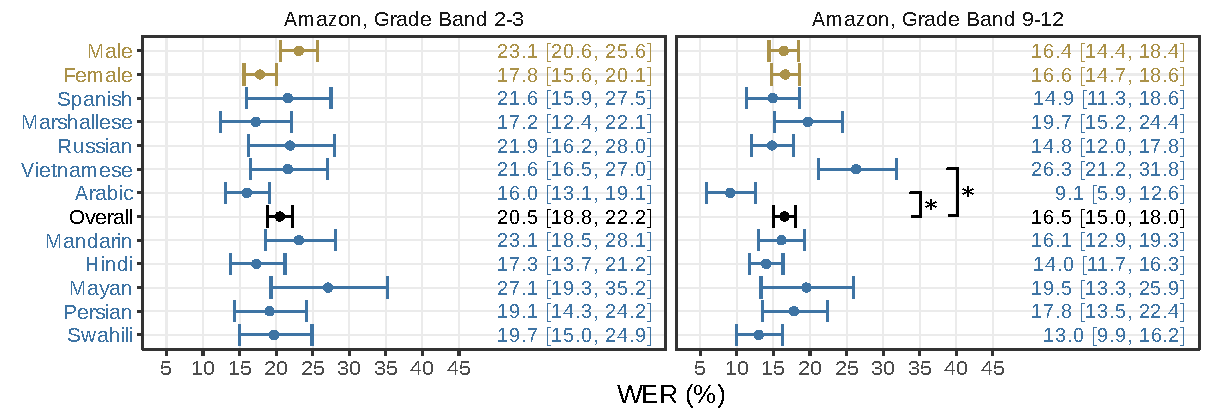
\includegraphics[width=6.5in]{figures/20230513_adj_werPlot_sigBars_aws.pdf}
    \label{wer_aws}
{Note: Overall WER appear in black, and disaggregated WER appear in gold (gender) and blue (L1); whiskers indicate 95\% confidence intervals; brackets with asterisks indicate statistically significant pairwise comparisons. \par}
\end{figure}

\subsection{Gender biases}

With respect to gender, results show no statistically significant differences between male and female WERs. Note that, while female speakers tended to have lower WERs, these differences were statistically significant using B-H adjusted p-values.

\subsection{L1 biases}

Results show two statistically significant differences based on speakers’ L1. Native Vietnamese speakers had a higher WER, on average, compared to other L1s. In contrast, native Arabic speakers had a lower WER compared to other L1s. 

\subsection{Age differences}

There were also differences in WER based on speakers' grade band. Although it does not make sense to characterize these differences as biases, in the same way as gender or L1, yet they may be relevant to further studies of automated English speaking assessment.

The WER of children (grades 2-3) were found to be significantly higher than WERs of young adults (grades 9-12). For Amazon, WERs were 20.5\% [18.8\%, 22.2\%] and 16.5\% [15.0\%, 18.0\%].

\subsection{Differences across services and datasets}

Although not the focus of Study 1, I compared WER across automated transcription service (Appendix \ref{sec:appendix_wer}), and repeated analyses on a public dataset (Appendix \ref{sec:appendix_l2}). These additional analyses provide evidence that the results of Study 1 are robust. In particular, speakers of Vietnamese L1 backgrounds have higher WERs in L2-ARCTIC data, and across all three automated transcription services. Arabic speakers, however, do not have a lower WER for L2-ARCTIC, and the difference is not as extreme for Microsoft and Google as it is for Amazon. 

\section{Study 1 Summary}

The main finding of Study 1 is that there are indeed biases in automated transcription of examinees’ speech for certain L1 backgrounds. Transcription was less accurate for young adults (grade band 9–12) whose L1 was Vietnamese. This finding is also consistent with a prior study of adult L2 English speech \citep{chan2022training}. It is interesting to note that this bias was not present for younger examinees (grade band 2–3). Findings from Study 1 were focused on Amazon’s automated transcription service, since Amazon was selected as the main automated transcription service for Studies 2 and 3; however, similar biases were found for Microsoft and Google (Appendix \ref{sec:appendix_wer}). 

Although our analyses did not detect gender bias, other studies have found that gender bias poses a major problem in ASR \citep{hutiri2022}. With a larger sample size, it would be possible to calculate more accurate WER estimates and to determine the size and direction of gender-based differences. 

Given that I do not have access to the training data or models used in developing these services, I was unable to identify the source of the biases or attempt to mitigate them. Other researchers, however, point out that biases exists at every stage of the ASR development pipeline \citep{hutiri2022, suresh2021framework}.

Although Study 1 highlights specific L1 biases in ASR systems, it is insufficient in determining if and how these biases impact examinees' test scores in automated English speech assessment. Study 2, however, brings some evidence to bear on this question. 



\chapter{Study 2: Gender and L1 Bias in Human and Automated Scores in English Speaking Assessment}

In L2 English speaking assessment, pretrained large language models (LLMs) such as BERT can score constructed response items as accurately as human raters. Less research has investigated whether LLMs perpetuate or exacerbate biases, which would pose problems for the fairness and validity of the test. Study 2 examines gender and native language (L1) biases in human and automated scores, using an off-the-shelf (OOS) BERT model. Analyses of bias focus on differential item functioning (DIF). Results show that, with respect to examinees’ L1 background in grade band 9–12, there is a moderate amount of DIF, and this DIF is higher when scored by an OOS BERT model. In practical terms, the degree to which BERT exacerbates DIF is very small. Additionally, there is more DIF for longer speaking items and for older examinees, but BERT does not exacerbate these patterns of DIF. 

\section{Study 2 Overview} 

Study 2 is designed to analyze gender and L1 biases in human and automated scores. For the automated scoring model, I use an off-the-shelf (OOS) pretrained Bidirectional Encoding Representation using Transformers (BERT) because of its seminal status in the field \citep{devlin2018} and the fact that it remains a focus of study in educational assessment (Evanini/Wang). Bias is quantified using differential item functioning (DIF). I describe specific patterns of DIF in human scores, and determine whether or not BERT exacerbates DIF. 

This study is designed to address four specific research questions:

\begin{enumerate}
	\item Compared to human scores, do automated scores increase overall DIF with respect to gender or L1? 
	\item Does DIF increase with item length and, if so, is this exacerbated by automated scores?
	\item Is DIF higher for older examinees and, if so, is this exacerbated by automated scores?
	\item Which specific groups of examinees are (dis)advantaged most, and do automated scores exacerbate this (dis)advantage?
\end{enumerate}

\section{Study 2 Methods}

The data source and sample used in analyses were described previously (Section \ref{sec:meth_sample}), as were automated transcription processes (Section \ref{meth_auto_transcribe}), methods used to quantify DIF (Section \ref{meth_dif}), p-value adjustment (Section \ref{meth_bh}), and models and training procedures (Section \ref{sec:meth_bert}). Study 2 used off-the-shelf (OOS) BERT models provided by Huggingface \citep{wolf_transformers_2020}. 

\subsection{Performance metrics}

In terms of performance, OOS BERT models nearly achieved parity with human raters for items 1–2 (for both grade bands), and BERT performed as well as (and, in grade band 9–12, outperformed) human raters for item 3. Table \ref{bert_perf} reports the performance of each of the six BERT models in terms of accuracy, correlation, and quadratic weighted kappa, as compared to human-human agreement (derived from doubly-scored responses). 

\begin{table*}[ht]
\centering
\caption{\label{bert_perf} \raggedright Performance of off-the-shelf BERT scoring models for items 1–3, compared to human-human agreement, with respect to accuracy, correlation ($r$), and quadratic weighted kappa (QWK)}
\small  % comment out this line if wanted bigger font size
\begin{tabular}{lccccccccccccccccc}
\toprule
    & \multicolumn{8}{c}{\textbf{Grade Band 2-3}} & \multicolumn{1}{c}{ } & \multicolumn{8}{c}{\textbf{Grade Band 9-12}} \\
    \cline{2-9}
    \cline{11-18}
    & \multicolumn{2}{c}{\textbf{Acc.}} & & \multicolumn{2}{c}{\textbf{r}} & & \multicolumn{2}{c}{\textbf{QWK}} & \multicolumn{1}{c}{ } & \multicolumn{2}{c}{\textbf{Acc.}} & & \multicolumn{2}{c}{\textbf{r}} & & \multicolumn{2}{c}{\textbf{QWK}} \\
\cline{2-3}
\cline{5-6}
\cline{8-9}
\cline{11-12}
\cline{14-15}
\cline{17-18}
    \textbf{Item} & \textbf{H} & \textbf{B} & & \textbf{H} & \textbf{B} & & \textbf{H} & \textbf{B} & & \textbf{H} & \textbf{B} & & \textbf{H} & \textbf{B} & & \textbf{H} & \textbf{B} \\
    \midrule
1 & .911 & .896 & & .793 & .713 & & .792 & .713 & & .929 & .904 & & .920 & .895 & & .920 & .895 \\
2 & .756 & .685 & & .898 & .861 & & .898 & .859 & & .728 & .700 & & .911 & .910 & & .911 & .909 \\
3 & .614 & .618 & & .834 & .834 & & .834 & .829 & & .694 & .707 & & .841 & .885 & & .609 & .884 \\
    \bottomrule
    \end{tabular}
{\raggedright \newline \newline  Note: "H" refers to human-human comparisons (i.e. rater 2 compared to rater 1). The number of observations that were scored by two human raters ranges from 1,567–1641 for Grade Band 2–3, and from 1,254–1,293 for Grade Band 9–12. "B" refers to human-BERT comparisons (i.e. BERT compared to rater 1). The number of observations in the testing sets were 4,185 for Grade Band 2–3, and 3,306 for Grade Band 9–12. \par}
\end{table*}

\section{Study 2 Results}

\subsection{BERT increases DIF for L1}
\label{res_rq1}

Overall, BERT-based automated scores increased DIF (to a very small degree) with respect to L1 in Grade Band 9–12. Although this difference is visible across all items in Grade Band 9–12, Item 3 carries the largest difference between human and automated scores. 

\subsubsection{Overall DIF of human scores}

Results revealed a moderate amount of DIF in human ratings based on examinees’ L1 in Grade Band 9–12. This result is visualized in Figure \ref{fig:zabs_ovr}, which shows a gray bar (representing human scores) extending into the yellow (“moderate” DIF) region of the chart ($z_{abs} = .196, CI_{95\%} = [.170, .222], p = 5.4 \cdot 10^{-48}$). Additionally, there was non-zero DIF based on L1 in Grade Band 2–3, and non-zero DIF based on gender in Grade Band 9–12; however, the effect sizes of these quantities were weak.

\begin{figure}[h]
    \centering
    \caption{Estimates of DIF by gender and L1 over all 3 items for grade bands 2–3 and 9–12.}    
%\hspace{-.6cm}
    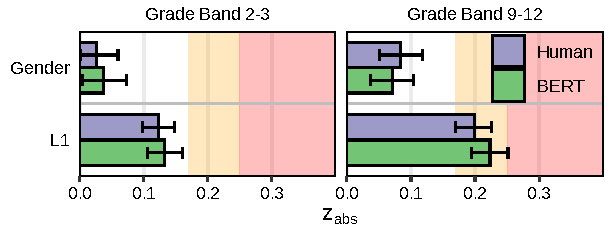
\includegraphics[width=4.5in]{figures/20230504_ETS-DIF_BERT_zabs_ovr_edit.pdf}
    \label{fig:zabs_ovr}
	{\newline Note: Error bars indicate 95\% confidence intervals. Yellow shaded regions correspond to moderate DIF, and red shaded regions correspond to strong DIF. \par}
\end{figure}

\subsubsection{Human vs. BERT overall DIF}

Overall DIF of automated scores was highly similar to human scores. As seen in Figure \ref{fig:zabs_ovr}, green bars (representing BERT scores) are nearly commensurate with gray bars (representing human scores), with mostly overlapping 95\% confidence intervals. Yet, there was significantly more DIF in BERT scores compared to human scores with respect to L1 in Grade Band 9–12 ($\Delta z_{abs} = .025, CI_{95\%} = [.011, .039], p = 3.3 \cdot 10^{-4}$). In practical terms, however, an effect size of 0.025 standard deviations is very small. 

\subsubsection{Human vs. BERT individual item DIF}

In addition to overall DIF, we examined DIF of each individual item. Figure \ref{fig:zabs_itm} presents DIF of human and automated scores, for gender and L1, across Items 1–3, for each grade band. Human and automated scores are again quite consistent. For Grade Band 9–12, L1 DIF tends to be higher across all items; however, only Item 3 reaches statistical significance ($\Delta z_{abs} = .032, CI_{95\%} = [.010, .055], p = 3.3 \cdot 10^{-3}$). An effect size of 0.032 is very small.

\begin{figure}[h]
    \centering
    \caption{Estimates of DIF by gender and L1 for each of the 3 speaking items in grade bands 2–3 and 9–12.}    
%\hspace{-.6cm}
    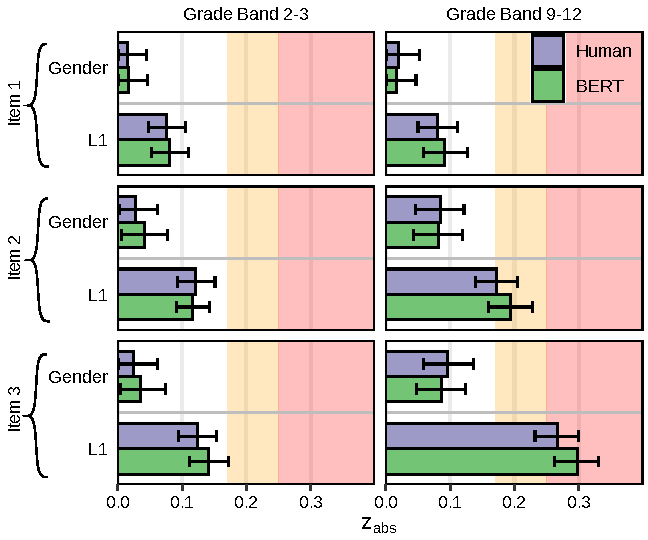
\includegraphics[width=5in]{figures/20230504_ETS-DIF_BERT_zabs_itm_edit.pdf}
    \label{fig:zabs_itm}
	{\newline Note: Error bars indicate 95\% confidence intervals. Yellow shaded regions correspond to moderate DIF, and red shaded regions correspond to strong DIF. \par}
\end{figure}

\subsection{DIF increases with item length}

Longer speaking items tended to exhibit more DIF than shorter speaking items. Automated scores, however, do not exacerbate this trend. 

In terms of item length, Item 3 was longer than Item 2, which was in turn longer than Item 1. Figure \ref{fig:zabs_itm} shows that DIF, too, generally increased in magnitude across items 1–3. Table \ref{itm_diff} presents the specific values of $\Delta z_{abs,ij}$ for all three item comparisons (corresponding to combinations of Item $i \neq j$) for each grade-band. 

\begin{table*}[ht]
\centering
\caption{\label{itm_diff}
Differences in DIF between longer and shorter items, within each grade band, based on human ratings.}
\small  % comment out this line if wanted bigger font size
\begin{tabular}{lccccccc}
\toprule
    & \multicolumn{3}{c}{\textbf{Grade Band 2-3}} & \multicolumn{1}{c}{ } & \multicolumn{3}{c}{\textbf{Grade Band 9-12}} \\
    \cline{2-4}
    \cline{6-8}
    \textbf{Factor} & \textbf{2 - 1} & \textbf{3 - 1} & \textbf{3 - 2} & & \textbf{2 - 1} & \textbf{3 - 1} & \textbf{3 - 2} \\
    \midrule
    \multirow{2}*{Gender} & .012 & .010 & -.002 & & .065 * & .078 * & .013 \\
    & [-.030, .051] & [-.029, .049] & [-.042, .039] & & [.021, .110] & [.031, .116] & [-.032, .055] \\
    \multirow{2}*{L1} & .046 * & .053 * & .006 & & .087 * & .184 * & .097 * \\
    & [.009, .085] & [.010, .093] & [-.035, .046] & & [.043, .130] & [.139, .226] & [.056, .138] \\
    \bottomrule
    \end{tabular}
{\raggedright \newline \newline  Note: "*" indicates that an estimate is statistically significant using B-H adjusted p-values. 95\% confidence intervals are presented in square brackets. \par}
\end{table*}

Although longer items tend to have more DIF, this general trend was not uniformly consistent across factors and grade-bands. Specifically, the trend was less consistent for gender: There were no statistically significant differences in Grade Band 2–3; and in Grade Band 9–12, Item 3 did not have more DIF than Item 2 at a statistically significant level. Additionally, for Grade Band 2–3, Item 3 did not have significantly more DIF than Item 2.

In order to determine if item-item differences were exacerbated by automated scoring, we computed second-order differences, $\Delta \Delta z_{abs}$. None of these values, however, were statistically significant. We conclude that the pattern of longer-items producing more DIF is consistent for both human and automated raters. 

\subsection{DIF is higher for older examinees}

In general, there is more DIF for older examinees (in Grade Band 9–12) compared to younger examinees (in Grade Band 2–3). Automated scores, however, do not exacerbate this trend.

There is significantly more DIF for Grade Band 9–12 compared to 2–3, in terms of both gender and L1. This trend can be seen clearly in Figure \ref{fig:zabs_itm}. Based on bootstrapped estimates for gender, $\Delta z_{abs} = .059$ ($CI_{95\%} = [.011, .100], p = 4.9 \cdot 10^{-3}$); and for L1, $\Delta z_{abs} = 0.082$ ($CI_{95\%} = [0.047, 0.120], p = 3.8 \cdot 10^{-6}$). 

When we examine individual items, this trend is present for items that are medium–long (Items 2 and 3) but not for short items (Item 1). Visually, this can be seen in Figure \ref{fig:zabs_itm}. Numerically, this is presented for human ratings in Table \ref{gr_diff}. 


\begin{table}[htbp]
\centering
\caption{\label{gr_diff}
Differences in DIF between grade-bands, based on human ratings, for each of the three speaking items. }
\small  % comment out this line if wanted bigger font size
\begin{tabular}{lccc}
\toprule
\textbf{Factor} & \textbf{Item 1} & \textbf{Item 2} & \textbf{Item 3} \\
\midrule
Gender & 0.004 [-0.035, 0.043] & 0.058 * [0.006, 0.104] & 0.071 * [0.02, 0.119] \\
L1 & 0.005 [-0.037, 0.048] & 0.05 * [0.006, 0.095] & 0.144 * [0.098, 0.189] \\
\bottomrule
\end{tabular}
{\newline \newline Note: "*" indicates that an estimate is statistically significant using B-H adjusted p-values. 95\% confidence intervals are provided in square brackets. \par}
\end{table}

In order to determine if differences between grade-bands were exacerbated by automated scoring, we computed second-order differences, $\Delta \Delta z_{abs}$. None of these values, however, were statistically significant. We conclude that the trend of greater DIF in older examinees is consistent for both human and automated raters. 

\subsection{Severity of DIF depends on L1 and grade band}

The magnitude and quantity of DIF varied by L1 background, and patterns were generally not consistent across grade-bands. Figure \ref{fig:z_ovr} depicts the magnitude and direction of DIF for gender and all L1 groups. For Grade Band 2–3, native speakers of Marshallese and Mayan languages showed evidence of moderate–strong DIF for human and BERT scores. DIF was negative for both L1 groups, indicating that these examinees fared worse on speaking items than their (equally-proficient) Spanish-speaking counterparts. 

\begin{figure*}[t]
    \centering
    \caption{Estimates of direction and magnitude of overall DIF.}
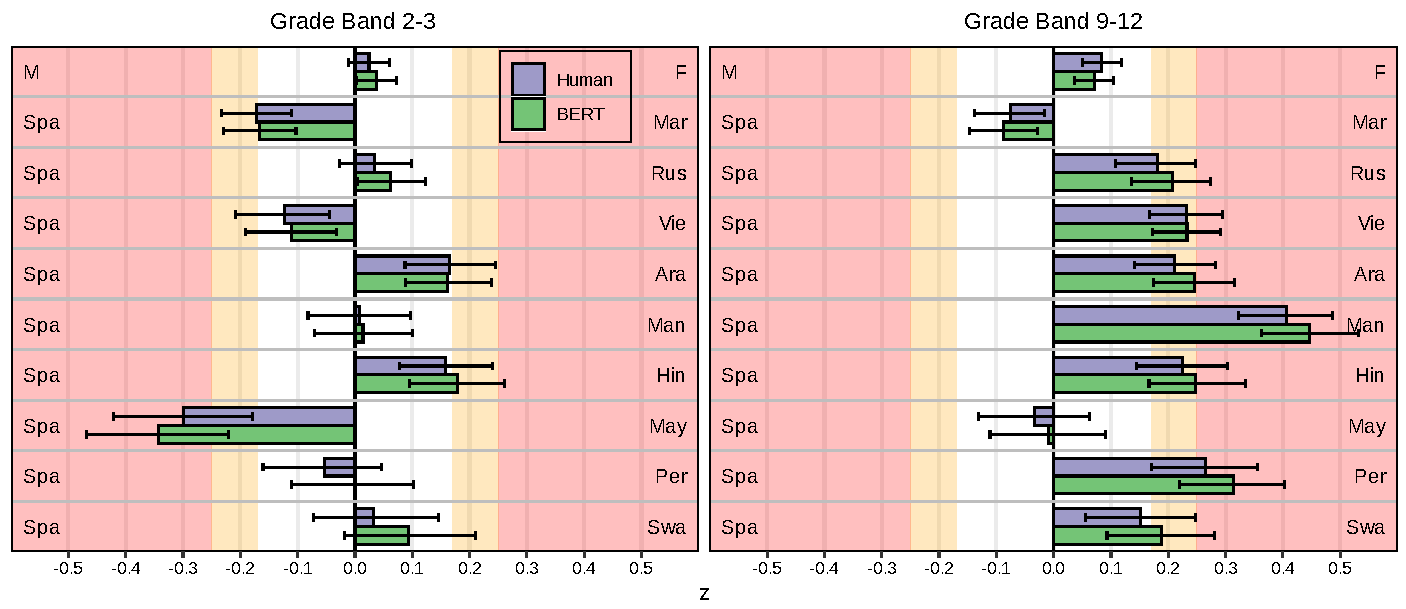
\includegraphics[width=6.5in]{figures/20230504_ETS-DIF_BERT_z_ovr_edit.pdf}   
    \label{fig:z_ovr}
{\newline Note: Error bars indicate 95\% confidence intervals. Yellow shaded regions correspond to moderate DIF, and red shaded regions correspond to strong DIF. Reference groups are listed on the left of each chart (M = Male, Spa = Spanish); focal groups are listed on the right (L1 groups are abbreviated by the first three letters). DIF in the positive direction indicates that the focal group is favored. \par}
\end{figure*}

In Grade Band 9–12, examinees of nearly all L1 backgrounds fared better than native Spanish speakers. In this case, speaking items tended to disadvantage members of the reference group (i.e. examinees with Spanish L1 backgrounds). 

As with preceding analyses, DIF based on BERT scores aligned closely with DIF based on human scores. Although results showed that BERT exacerbated DIF in L1 as a whole (Section \ref{res_rq1}), analyses of individual L1 groups did not reveal any statistically significant differences between human and BERT scores. We also did not find any statistically significant differences between human and BERT scores when examining DIF at the individual item level (Appendix \ref{sec:appendix_z_itm}). 

\section{Study 2 Summary}

\subsection{Main findings}

Analysis of differential item functioning (DIF) revealed specific patterns of biases in human and automated scores of English speaking assessment. With respect to human scores, I found that there was more DIF for older examinees and for longer items. Based on commonly accepted standards regarding effect size, there was a moderate amount of overall DIF in grade band 9–12 based on examinees’ native language (L1) backgrounds. Automated scores generated by off-the-shelf BERT closely matched human scores, yet BERT was found to exacerbate overall DIF for grade band 9–12 based on examinees’ native language (L1). The degree to which BERT exacerbated bias, however, was very small.

\subsection{Sources of DIF}

Although our findings do not confirm any causes of DIF, they do allow us to rule out several possibilities. 

\subsubsection{Transcription (in)accuracy}

Study 1 showed that there were discrepancies in word error rate (WER) of automated transcription based on L1. Specifically, automated transcription struggled with speakers of Vietnamese L1 backgrounds. Yet given the close correspondence between human and automated scores—for all examinees, not just Vietnamese examinees—it appears unlikely that transcription inaccuracies engendered lower or higher scores. 

\subsubsection{Implicit bias}

Our automated scoring system was based exclusively on transcripts of examinees’ speech. No phonic information was used in the automated scoring process. It is notable, then, that there was no mitigation of DIF in automated scores using a text-based BERT model. In other words, removal of acoustic input did not reduce bias. From this, we can conclude that examinees with \emph{identical} (transcribed) responses could not have received higher or lower scores, on average, based on gender or L1. 

Although text-based automated scores did not mitigate bias, this does not necessarily imply that human raters are unaffected by implicit bias. It is possible, for instance, that examinees with different accents also have different (transcribed) responses, which still affect human judgment. 

\subsection{Accuracy and DIF}

As the performance of automated scoring improves to match (or exceed) that of human raters, one might have expected the magnitude of DIF to also match (or potentially reduce) that of human raters. Contrary to expectation, for longer speaking items, automated scores exceeded the performance of human raters yet increased DIF. More research is needed to determine the relationship between performance and DIF. 



\chapter{Study 3: Mitigating Gender and L1 Bias in Automated English Speaking Assessment}

Having examined patterns of bias in Study 2, it was found that there is a moderate degree of differential item functioning (DIF) for grade band 9–12, based on examinees’ native language (L1). Drawing from a new body of research in machine learning known as debiasing, Study 3 explores the possibility of reducing DIF. I compare two different debiasing approaches: The adversarial approach, which surgically removes aspects of gender or L1 from examinees’ responses; and the shrinkage approach, which averages automated scores with examinees’ expected scores (ES). Results show that the adversarial approach fails to reduce DIF, producing identical scores to off-the-shelf (OOS) BERT models. Although the shrinkage approach uniformly reduces DIF, it does so at the expense of item information. 

\section{Study 3 Overview}

As a growing field in machine learning, debiasing is focused on making predictions more equitable with respect to protected attributes \citep{elazar2018adversarial}. In many contexts, the prediction task (in this case, English speaking scoring) may be intertwined with protected attributes (i.e., gender or L1), and it is the goal of debiasing to untangle this association and prevent protected information from affecting task predictions. Sometimes the association between the task and the protected attribute is referred to as leakage, in the sense that information in the prediction function leaks information about the protected class. There are numerous techniques that have been proposed and applied toward specific tasks, but because it is a relatively new field, there is little consensus as to which techniques are most effective \citep{sun2019mitigating}. 

Debiasing techniques have not been applied to English speaking assessment, yet they may offer a solution to reduce biases (such as the patterns of DIF enumerated in Study 2). It may be possible to reduce biases introduced by LLMs, and perhaps even to reduce bias below what is seen in human rater scores. \citet{sun2019mitigating} review a number of techniques to debiasing, and organize these by methodological approach. In Study 3, I apply two of these techniques toward mitigating gender and L1 biases in automated English speaking assessment, and discuss the relative merits and weaknesses of each. 

\subsection{The adversarial approach}

The adversarial approach is characterized by predicting the protected class, and then preventing the model from using this information in task predictions. In one application of this technique, \citet{wang2019balanced} first trained a model to predict gender and, subsequently, during task training, reversed the optimization function so that the model unlearned its ability to predict gender. 

This approach is appealing because it attempts to remove biases specific to the protected attributes. This approach is surgical in removing only the parts of the prediction function that are related to the protected attributes. Aspects of the protected attribute that are related to the task function are actively unlearned. In image recognition, this is analogous to removing facial details or hair styles that might be related to gender. With respect to English speaking assessment, this approach would (in theory) unlearn aspects of the scoring function that are related to gender or L1. 

\subsection{The constrained prediction approach}

Another approach is constrained prediction, which involves altering predictions after training is completed. One way of doing this is to alter the probability distributions so that each protected attribute has equal odds of receiving the same prediction \citep[e.g.][]{yatskar2016situation}. The method that I employ in Study 3 is to use a shrinkage estimator \citep{fourdrinier2018shrinkage}, which is tailored specifically to shrink estimates towards zero DIF. The specific condition that shrinks predicted scores towards zero DIF is when examinees’ scores are exactly equal to their expected scores, based on their responses to non-speaking items. (Expected scores are described in greater detail in Section \ref{sec:meth_es}).

subsection{Research questions and study design}

Study 3 explores two approaches of debiasing gender and L1 in English speaking assessment. The specific research questions I address are:

\begin{enumerate}
	\item Does the adversarial approach reduce overall DIF, based on gender or L1?
	\item What are the causes of the adversarial model’s success or failure?
	\item Does a constrained prediction approach reduced overall DIF, based on gender or L1?
	\item What are the causes of the constrained prediction model’s success or failure?
\end{enumerate}

In the Summary, I also consider the advantages and limitations afforded by each approach, and I suggest possible developments and/or further research that could redress those limitations. 

\section{Study 3 Methods}

The data source and sample used in analyses were described previously (Section \ref{sec:meth_sample}), as were automated transcription processes (Section \ref{meth_auto_transcribe}), methods used to quantify DIF (Section \ref{meth_dif}), p-value adjustment (Section \ref{meth_bh}), and models and training procedures (Section \ref{sec:meth_bert}). Consistent with Study 2, Study 3 uses off-the-shelf BERT models provided by Huggingface \citep{wolf_transformers_2020}, as well as modified BERT models; modifications were made with Pytorch \citep{paszke_pytorch_2019}, based on original models provided by Huggingface \citep{wolf_transformers_2020}.

\subsection{Adversarial models}

Debiasing models included three classifications heads, corresponding to score, gender, and L1 predictions. Cross entropy loss was calculated for each classification head. Before taking each optimization step, losses were combined so as to reduce bias. Following the example of \citet{wang2019balanced}, the final objective is, 

$$
L_p = \sum_{(X_i, h_i, Y_i)} [L(p(X_i), Y_i) - \lambda_g L_{c_g}(c_g(h_i), g_i) - \lambda_l L_{c_l}(c_l(h_i), l_i)] 
$$

where $p(X_i)$ are the predicted scores, $Y_i$ are the actual scores, and $c_g(h_i)$ and $c_l(h_i)$ are "critics," i.e., functions that predict protected classes (i.e. gender and L1, respective) from BERT’s contextual token embedding (or "pooled output"), $h$. $\lambda_g$ and $\lambda_l$ represent hyperparameters to weight the importance of the gender and L1 critic, respectively. 

\subsection{Shrinkage models}

The DIF shrinkage approach computes examinees scores from a weighted average of (1) examinees’ predicted scores, using regression BERT models, and (2) examinees' expected scores, based on their responses to non-speaking items. Expected scores are described in greater detail in Section \ref{sec:meth_es}. 

Regression BERT models are off-the-shelf (OOS) BERT models. Instead of predicting score categories using cross-entropy loss, however, these models are trained to predict a single, continuous score using mean squared error loss. Thus, most predicted regression scores were non-integers. 

Regression scores (RS) were combined with examinees’ expected scores (ES), at varying weights (or proportions), to produce regularized scores. Study 3 includes five different weighting conditions: $1 RS + 0 ES$, $.75 RS + .25 ES$, $.5 RS + .5 ES$, $.25 RS + .75 ES$, and $0 RS + 1 ES$. Combined scores were rounded to the nearest whole integer, in order to remain consistent with human raters. 

\subsection{Expected score estimates}
\label{sec:meth_es}

Based on examinees’ responses to non-speaking items, expected score (ES) was computed for responses to each item in examinees’ respective grade bands. That is, each examinee had three ESs, corresponding to items 1–3. ES is a function of non-speaking proficiency, $\theta$, and IRT item parameters, $a$ and \textbf{b}. More specifically, for examinee $i$, responding to item $j$, across all possible scores, $u$, $ES_{ij} = E[U=u|\theta_i, a_j, \textbf{b}_j]$. For computation of $\theta$, see Section \ref{meth_dif}. With respect to item parameters of items 1–3, items were modeled using the graded response model \citep{samejima1997graded} and computed using flexMIRT \citep{cai2012flexmirt}, based on the responses of all examinees in the sample. 

\section{Study 3 Results}

\subsection{The adversarial approach}

The adversarial model failed to remove overall DIF, by gender or L1, over all three items, in either grade band 2–3 or 9–12. Figure \ref{advBERT_zabs_ovr} compares overall DIF based on human scores (gray) to off-the-shelf BERT (green) and the adversarial BERT model (dark green). Although there were minor differences between off-the-shelf BERT and adversarial BERT, none of these differences ($z_{abs}$) were statistically significant. Differences may be attributed to noise (e.g. slightly different starting values). 

\begin{figure}[h]
    \centering
    \caption{Comparisons of overall DIF across human, off-the-shelf BERT, and adversarial BERT, by gender and L1 over all 3 items for grade bands 2–3 and 9–12.}    
%\hspace{-.6cm}
    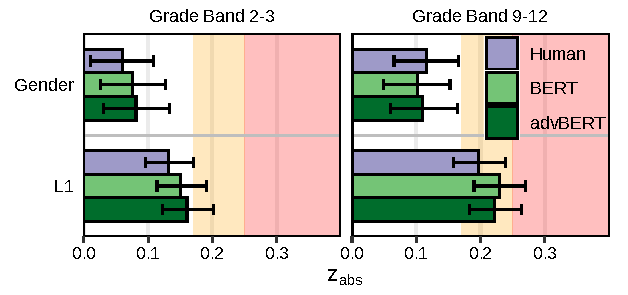
\includegraphics[width=4.5in]{figures/20230517_ETS-DIF_advBERT_zabs_ovr_edit.pdf}
    \label{advBERT_zabs_ovr}
	{\newline Note: BERT represents the off-the-shelf BERT model, and advBERT represents the adversarial BERT model. Error bars indicate 95\% confidence intervals. Yellow shaded regions correspond to moderate DIF, and red shaded regions correspond to strong DIF. Estimates of magnitude of L1 DIF are the average $z_abs$ for all 9 focal groups. \par}
\end{figure}

There were also no statistically significant differences between off-the-shelf BERT and adversarial BERT when examining the direction and magnitude of overall DIF, based on gender or any individual L1 group (Figure \ref{advBERT_z_ovr}). Again, although there were minor discrepancies, none of the discrepancies ($\delta z$) were statistically significant.

\begin{figure}[h]
    \centering
    \caption{Comparisons of direction and magnitude of overall DIF across human, off-the-shelf BERT, and adversarial BERT, by gender and each L1 group for grade bands 2–3 and 9–12.}    
%\hspace{-.6cm}
    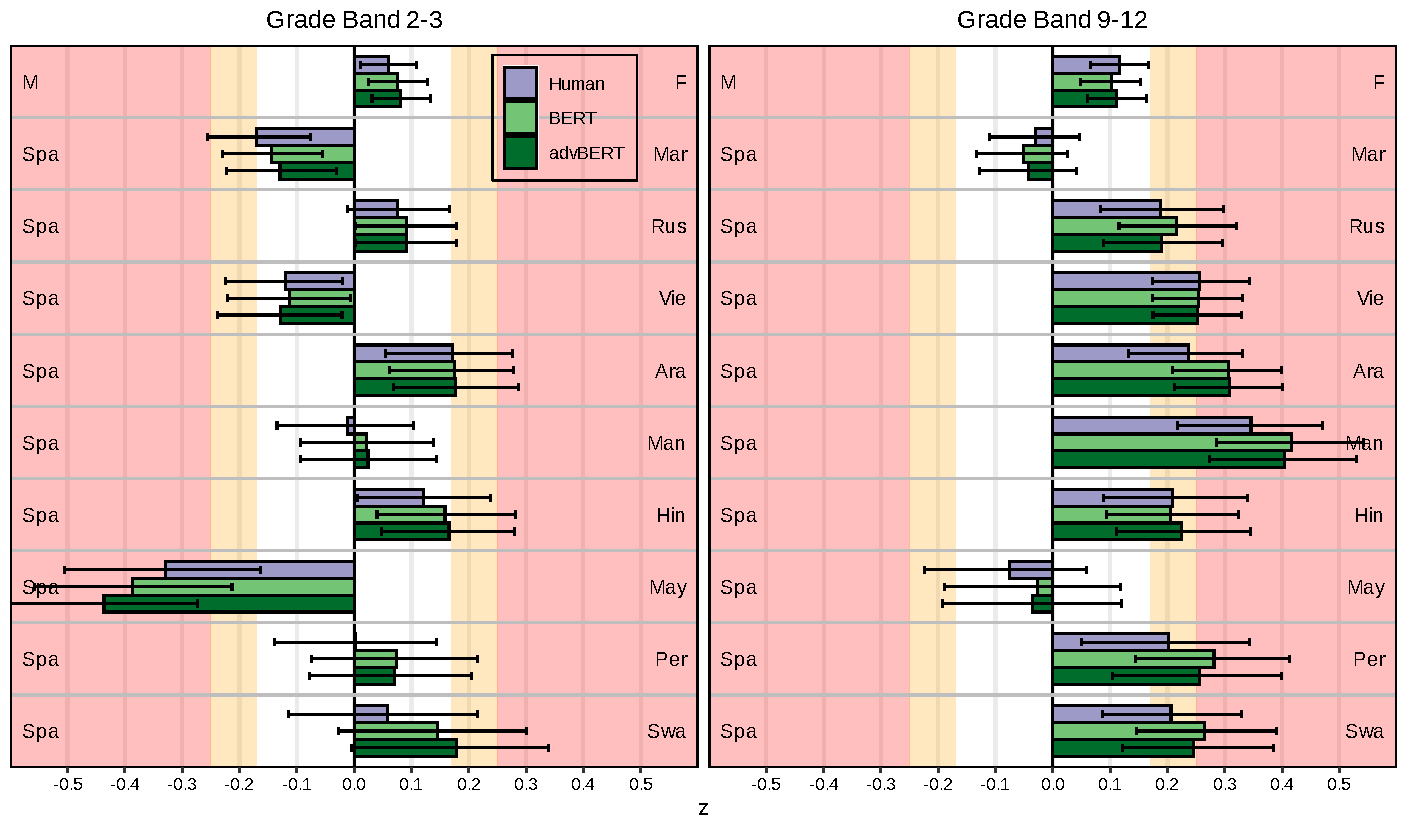
\includegraphics[width=6.5in]{figures/20230517_ETS-DIF_advBERT_z_ovr_edit.pdf}
    \label{advBERT_z_ovr}
	{\newline Note: BERT represents the off-the-shelf BERT model, and advBERT represents the adversarial BERT model. Error bars indicate 95\% confidence intervals. Yellow shaded regions correspond to moderate DIF, and red shaded regions correspond to strong DIF. Reference groups are listed on the left of each chart (M = Male, Spa = Spanish); focal groups are listed on the right (L1 groups are abbreviated by the first three letters). DIF in the positive direction advantages the focal group. \par}
\end{figure}

One of the reasons why the adversarial BERT model may not reduce DIF is that there is little to no leakage. Indeed, evidence suggests that there is little information about the protected attributes in examinees’ responses at all, let alone present in the score prediction function. In simpler terms, there are few differences in examinees’ responses, based on gender or L1. Figure \ref{heatmap_gend} presents the accuracy with which BERT predicted gender based on examinees’ responses for each of the 3 speaking items in grade bands 2–3 and 9–12. In both grade bands, there are many incorrect (i.e. off-diagonal) predictions. Indeed, the predictions are nearly random, suggesting that there is little signal of gender at all in examinees’ responses. In grade band 9–12, the majority of responses are predicted as male. 

\begin{figure}[h]
    \centering
    \caption{Confusion matrix of BERT predictions of gender for each of the 3 speaking items in grade bands 2–3 and 9–12.}    
%\hspace{-.6cm}
    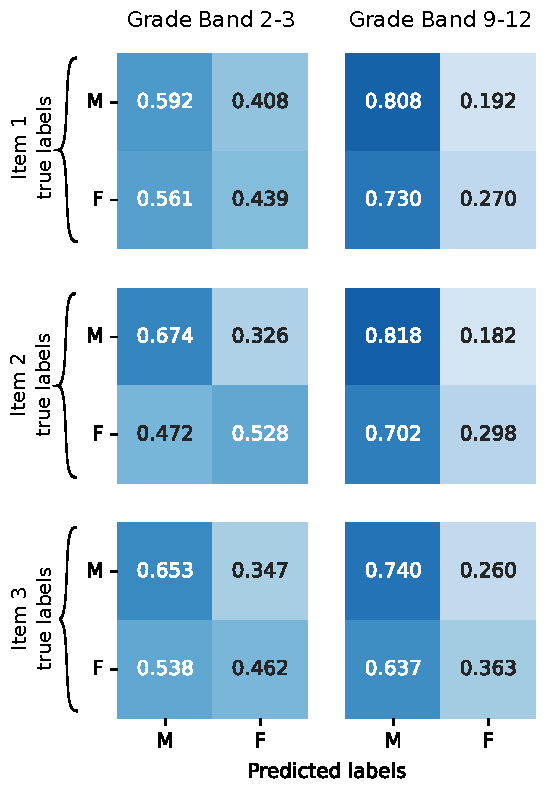
\includegraphics[width=3in]{figures/20230516_gender805_heatmap_edit.pdf}
    \label{heatmap_gend}
	{\newline Note: accuracy is conditioned on the true number of examinees within each gender. \par}
\end{figure}

With respect to predicting L1 group based on examinees’ responses, the situation is even more extreme than gender. For both grade bands, and across all three items, BERT makes the almost uniform prediction that examinees’ L1 is Spanish (Figure \ref{heatmap_lang}). Although the dominance of Spanish predictions is due to it being the largest L1 group, the lack of accurately predicting any other L1 group suggests there is not a moderate (let alone strong) signal in examinees’ responses based on L1. Note that analyses of confusion matrices do not control for score, which precludes the possibility of identifying more subtle differences in examinees’ responses. 

\begin{figure}[h]
    \centering
    \caption{Confusion matrix of BERT predictions of L1 group for each of the 3 speaking items in grade bands 2–3 and 9–12.}    
%\hspace{-.6cm}
    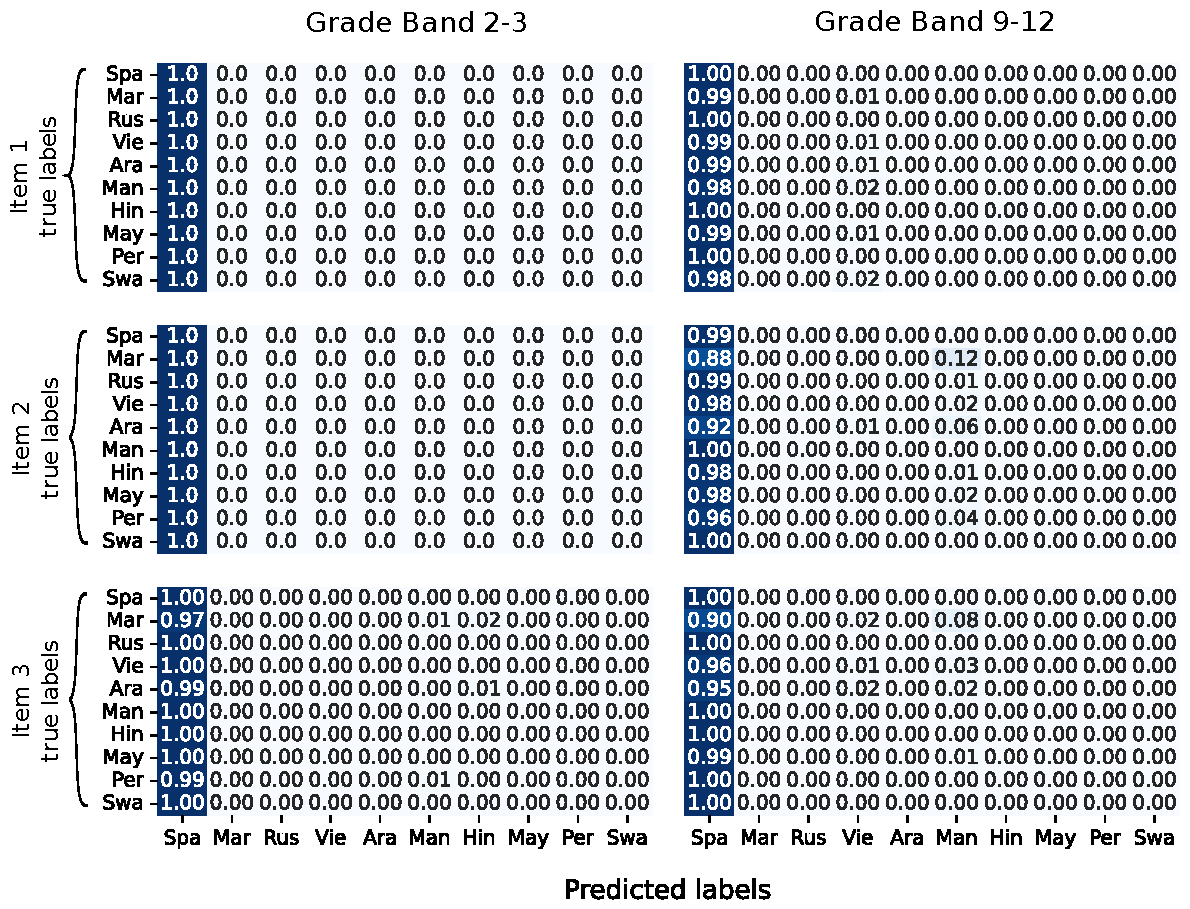
\includegraphics[width=6.5in]{figures/20230516_language805_heatmap_edit.pdf}
    \label{heatmap_lang}
	{\newline Note: accuracy is conditioned on the true number of examinees within each L1 group. \par}
\end{figure}

\subsection{The shrinkage approach}

Results indicate that shrinking BERT scores towards examinees’ expected scores (ES) reduces (and, in the extreme case, eliminates) DIF. The degree of reduction of DIF depends on the percentage of the weighted average apportioned to ES. If zero weight is apportioned to ES, then results are identical to patterns of DIF seen in Study 2. As a greater percentage of the score is apportioned to ES (i.e. 25\%, 50\%, and 75\%), there is a corresponding decrease in DIF. In the extreme case, when scores are exclusively determined by ES, DIF is eliminated. Recall that ES is based on examinees’ responses to non-speaking items (Section \ref{sec:meth_es}); thus, although DIF is eliminated when ES exclusively determines examinees’ scores, the items also fail to assess speaking. In the extreme case, "speaking" scores are based on non-speaking items, and examinees’ responses are taken into consideration at all. Although impractical, the extreme example is helpful in illustrating the downside of reducing DIF with the shrinkage model. 

Figure \ref{fig:shrinkBERT_zabs_ovr} depicts the inverse relationship between DIF and the weight apportioned to ES across five conditions. Darker shades of green correspond to higher weights apportioned to ES. It is clear that DIF decreases monotonically as a greater percentage of examinees’ speaking scores are determined by their ES. 

\begin{figure}[h]
    \centering
    \caption{Comparisons of overall DIF across human and five shrinkage BERT models, by gender and L1 over all 3 items for grade bands 2–3 and 9–12.}    
%\hspace{-.6cm}
    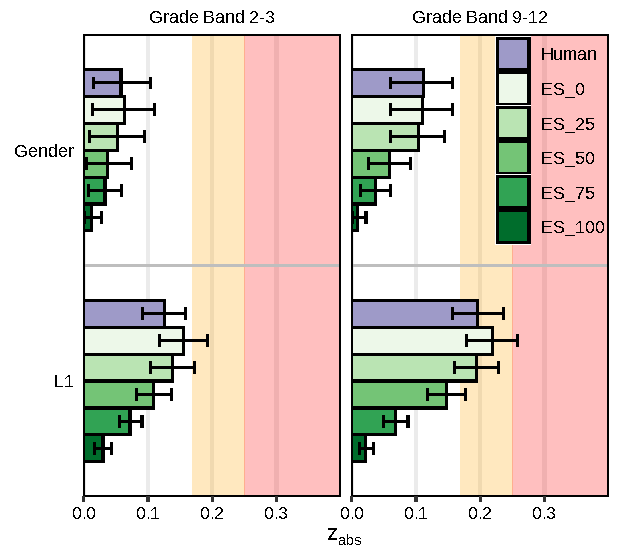
\includegraphics[width=4.5in]{figures/20230425_ETS-DIF_ES_zabs_ovr_edit.pdf}
    \label{fig:shrinkBERT_zabs_ovr}
	{\newline Note: ES stands for "expected score," and represents the percentage of weight given to expected score (in conjunction with regression BERT). Error bars indicate 95\% confidence intervals. Yellow shaded regions correspond to moderate DIF, and red shaded regions correspond to strong DIF. Estimates of magnitude of L1 DIF are the average $z_abs$ for all 9 focal groups. \par}
\end{figure}

DIF is also reduced (or eliminated) with the shrinkage model, regardless of direction or magnitude of DIF (Figure \ref{fig:shrinkBERT_z_ovr}). As above, Figure \ref{fig:shrinkBERT_z_ovr} presents DIF across five shrinkage models, corresponding to weight apportioned to ES, by gender and L1 group for grade bands 2–3 and 9–12. Although this study examines gender and L1, the shrinkage approach would eliminate DIF across all background factors. 

\begin{figure}[h]
    \centering
    \caption{Comparisons of direction and magnitude of overall DIF across human and five shrinkage BERT models, by gender and each L1 group for grade bands 2–3 and 9–12.}    
%\hspace{-.6cm}
    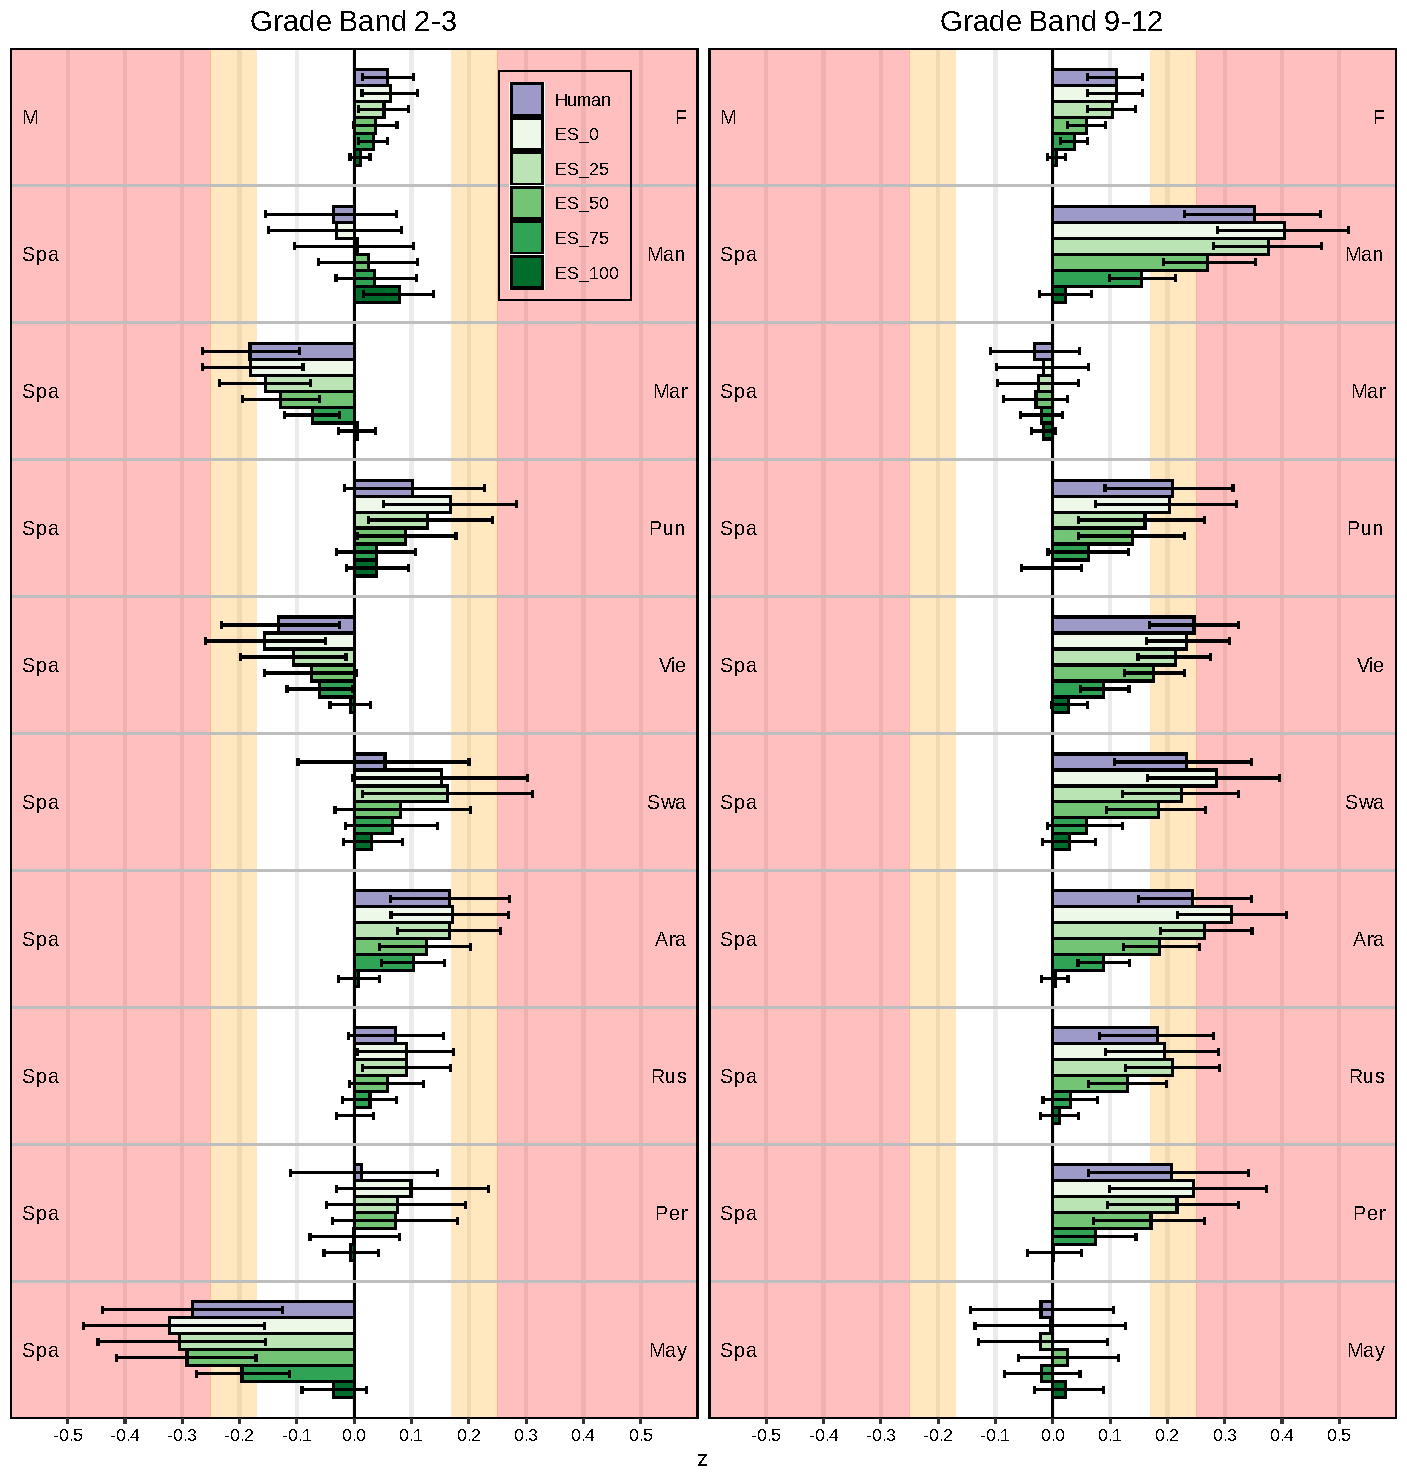
\includegraphics[width=6.5in]{figures/20230425_ETS-DIF_ES_z_ovr_edit.pdf}
    \label{fig:shrinkBERT_z_ovr}
	{\newline Note: ES stands for "expected score," and represents the percentage of weight given to expected score (in conjunction with regression BERT). Error bars indicate 95\% confidence intervals. Yellow shaded regions correspond to moderate DIF, and red shaded regions correspond to strong DIF. Reference groups are listed on the left of each chart (M = Male, Spa = Spanish); focal groups are listed on the right (L1 groups are abbreviated by the first three letters). DIF in the positive direction advantages the focal group. \par}
\end{figure}

\section{Study 3 Summary}
\label{sec:stdy3_sum}

\subsection{Limitations and further developments for the adversarial approach}

Speaking scores generated using the adversarial approach did not differ significantly from off-the-shelf BERT scores. One of the reasons the adversarial model failed to reduce DIF may be because examinees’ responses did not exhibit gender or L1 differences. Generally speaking, BERT was unable to predict gender or L1 from examinees’ responses. If this is indeed the case, then there would be no leakage to mitigate, and we would not expect the adversarial approach to mitigate DIF in the first place. 

Although results showed that the adversarial method was unable to reduce DIF, this could be less of a limitation of the method, and more of an indication that the method requires additional engineering. Specifically, although it was found that BERT was unable to predict gender or L1, the relationship between gender/L1 and response was not conditioned on examinees’ proficiency, which is critical in analyses of DIF. It is also possible that this lack of predictive power is due (in part) to the fact that the sample is imbalanced: There may be subtle differences in responses based on L1, but these are eclipsed by the fact that the vast majority of examinees have Spanish L1 backgrounds. More fine-grained analyses are needed to parse the relationship between responses and L1 background. Through data augmentation, it would be possible to rectify the imbalance between L1 group sizes. If these additional analyses do, in fact, reveal a relationship between examinees’ responses and L1, then it might reopen the possibility of mitigating DIF through adversarial means. 

Although there are other adversarial models, all would suffer from the same limitation of not being able to remove bias if there is leakage. \citet{zhang2018mitigating}, for instance, suggests projecting the task-specific gradient onto the orthogonal compliment of the protect attribute gradients during training. So long as the subspace is sufficiently restricted, this could prevent the model from learning to predict gender or L1 from responses, but only if there is relationship between gender/L1 and the response to begin with. 

\subsection{Limitations and further developments for the shrinkage approach}

Although the shrinkage approach reduces DIF (irrespective of magnitude, direction, or even background characteristic), it also reduces to a commensurate degree the information contained in test items. In the extreme case, examinees’ responses are determined exclusively by their non-speaking English proficiency. Thus, if applied uniformly to all speaking items, the shrinkage approach precludes the possibility of measuring speaking proficiency, and confounds the very purpose of the assessment. A more judicious application of the shrinkage approach, towards only those items exhibiting the most DIF, could be beneficial. Without knowing the source of DIF, however, it is impossible to know whether this more judicial application is still removing the most important components of speaking proficiency. This could very well be the case, given that longer speaking items exhibit more DIF. 

One possible extension of the shrinkage approach would be to specify further constraints so as to determine algorithmically the optimal weight to apportion to examinees’ expected scores. Study 3 analyzed five conditions of various weights; with additional specifications, the weight assigned would not be arbitrary, but determined a prior by some modified loss function. This addition might help clarify what is important, psychometrically. With more weight given to expected score, we reduce DIF, but we also reduce item information; it would make sense, then, to limit DIF while also maximizing some measure of item information—ideally, information that is orthogonal to non-speaking proficiency. 



\chapter{Discussion}

\section{Summary of Findings}

\subsection{Studies 1-3}

Study 1 analyzed the accuracy of a large-scale automated transcription service by comparing average word error rate (WER) of a subsample of examinees, disaggregated by gender and L1. Results showed no difference in accuracy based on gender, for either grade band. Yet, for grade band 9–12, examinees whose native language (L1) was Vietnamese tended to have less accurate transcripts, on average, while those with Arabic L1 backgrounds had more accurate transcripts. 

Study 2 examined patterns of differential item functioning (DIF) with respect to scores generated by human raters and by a common large language model known as BERT. Results revealed that, based on human rater scores, there was a moderate amount of overall DIF for grade band 9–12 based on examinees’ L1. Across both grade bands, there was more DIF for longer speaking items, and more DIF for older examinees (grade band 9–12) compared to younger examinees (grade band 2–3). BERT exacerbated DIF by a small amount, with respect to overall DIF for grade band 9–12 based on examinees’ L1. Yet BERT had identical patterns of DIF with respect to length of speaking items and age of examinees. Overall, BERT scores corresponded closely to human rater scores. 

Study 3 focused on two approaches aimed at mitigating DIF, the adversarial approach and the shrinkage approach. The adversarial approach produced scores that were not significantly different from the of-the-shelf BERT model used in Study 2. One possible reason for the failure of the adversarial model to mitigate DIF may be due to the lack of correspondence between examinees’ gender/L1 and their responses; however, additional research is needed to probe these relationships further. In contrast to the adversarial approach, the shrinkage approach did reduce DIF for gender and L1. The drawback of the shrinkage approach is that, as DIF is reduced, information regarding examinees’ speaking proficiency is also reduced. Without untangling the relationship between DIF and speaking proficiency, the shrinkage approach may undermine the very purpose of the assessment. 

\subsection{Overarching research goals}

This research project was designed in part around exploring two specific construct-irrelevant drivers of DIF, automated transcription bias and implicit bias. Evidence from Studies 1–2 rule out the possibility that automated transcription is the cause of DIF. And Studies 2–3 indicate that implicit bias is likely not the main issue. Yet there is room for further exploration of implicit bias, when additional data becomes available (see Section Sources of DIF). 

Another overarching goal of this research project was to explore debiasing techniques for the removal of DIF. It was especially of interest to explore adversarial methods capable of removing construct-irrelevant aspects of examinees’ responses (i.e. surgically removing aspects specific to gender or L1). Such a technique could be employed regardless of the main drivers of DIF. Unfortunately, this technique did not yield fruitful results, in part because there were no large differences in examinees’ responses based on gender or L1. 

\section{Sources of DIF}
\label{sec:disc_sources}

Results from Studies 1–3 allow us to rule out certain sources of DIF, and suggest possibilities for examining other sources more deeply. 

\subsection{Automated transcription}

Study 1 revealed that there were discrepancies in transcription accuracy that varied by L1. Yet Study 2 showed that there was very little room for these inaccuracies to affect scores. Rather, human rater scores and automated scores generated by BERT, when disaggregated by L1, were nearly identical; DIF was also nearly identical. Furthermore, we do not see DIF and accuracy trend in the same direction: examinees with Vietnamese L1 backgrounds have, on average, lower transcription accuracy, yet DIF seems to favor them over other L1 groups. Because of the tight correspondence between human and automated scores and human and automated DIF, automated transcription can be ruled out as a source of DIF. 

\subsection{Human rater bias}

Research on implicit bias suggested that human raters might judge certain accents more harshly than others. That is, examinees (of different L1 backgrounds) might give the same response, yet receive different scores. For instance, Spanish speakers and Mandarin speakers who both said "she put on her shoes" may receive different scores. Study 2, however, ruled out this possibility. If examinees had received different scores, then BERT (which takes text-only input) would have reduced DIF, which was not the case. Note that this finding is consistent with scoring rubrics, which focus on content of examinees’ responses, as opposed to aspects of fluency, such as pronunciation.

Based on Study 2, the possibility still remained, however, that examinees (of different L1 backgrounds) gave slightly different responses—that deserved the same scores—yet received different scores. For instance, consider the possibility that examinees of Spanish L1 backgrounds might have been more likely to say, "She put on her shoes," whereas examinees of Mandarin L1 backgrounds might have been more likely to say, "She was putting on her shoes." Although these responses deserve the same score, yet they may trigger implicit bias in human raters and be given different scores. Text only-based BERT might have continued to propagate these discrepancies. 

Results from Study 3, however, suggest that there was not a strong relationship between L1 and examinees’ responses. That is, BERT was not able to distinguish examinees whose L1 was Spanish versus Mandarin. This finding suggests that implicit bias—and even the more nuanced type of implicit bias described above—is unlikely. An important caveat to this claim is that, in the analysis of the relationship between response and L1, Study 3 did not control for examinees’ language proficiency (or, even more coarsely, human rater scores), which is critical in analyses of DIF. In examining whether human rater bias is a source of DIF, it is necessary not to compare examinees of Spanish and Mandarin L1 backgrounds as a whole, but only those examinees who deserve the same score. Unfortunately, exploring this possibility requires a great deal more data, since L1 groups would need to be partitioned by observed score, and some groups have little overlap in observed scores. 

\subsection{Sociocultural factors}

Item 3 is a science-related item, and item 2 for grade band 9–12 involves some quantitative reasoning. Depending on which countries students might have emigrated from, these types of content-related items might be easier for students with origins in countries where these concepts are covered \citep{huang2016exploring}. However, item 2 for grade band 2–3 still exhibits some DIF with respect to L1, and it is not related to science or quantitative reasoning. Furthermore, there are non-speaking science and quantitative reasoning items. Therefore, to pursue this possibility further, it would be beneficial to examine non-speaking items related to science or quantitative reasoning to see if similar patterns of DIF emerge. 

Study 2 revealed that examinees in grade band 9–12 who have Spanish L1 backgrounds tend to struggle with speaking items. There could be some sociocultural or socioeconomic cause, perhaps related to SES, migrant status, age of entry into the U.S. schooling system, or some other factor. Unfortunately, these data are not collected by all states, nor are they collected in the same way, which makes these analyses more difficult. 

There are other sociocultural factors that could be specific to speaking proficiency, such as opportunities or motivation to communicate with others \citep{derwing2013development}. However, exploring these factors would require data beyond what is available. 

\subsection{Feature bias}

Although feature biases are less salient when using deep learning models, manual features could be helpful in determining the sources of DIF. For instance, it has been shown that embedding layers of LLMs correlate with manually specified features \citep{ormerod2022mapping}. By examining intraclass correlation coefficients, it might be possible to ascertain which manual features are (or are not) associated with responses of each L1 group, providing additional leads for investigating sources of DIF. 

\subsection{Machine learning bias}

Given the close correspondence between scores generated by human raters and BERT, there is little room for machine learning bias. Nevertheless, Study 2 did find that BERT exacerbated DIF with respect to L1 in grade band 9–12. Even though the effect size is small, it is worth investigating whether or not this is due to modeling or training decisions. One possible avenue of research would be to experiment with different LLMs (besides BERT). In particular, it would be useful to repeat these analyses using a smaller LLM, such as Elektra or an ensemble of models \citep{ormerod2022short}. 

\subsection{Other biases}

The majority of non-speaking items are relatively easy, based on their IRT parameters. Research has suggested that easier items are more likely to exhibit DIF, since they may be more likely to draw on cultural knowledge \citep{santelices2010unfair}. If this is the case, then perhaps the non-speaking items do not constitute an appropriate set of anchor items. Although it contradicts research on implicit bias, it is possible that the speaking items are less biased than the non-speaking, anchor items. 

\citet{dorans2004examining} suggest that there is a relationship between impact and DIF. Although they suggest that this is tied to guessing behavior, which would not work the same way for construct response items, there might yet be a correlate for speaking items. For instance, it has been noted that speaking is the most difficult aspect of L2 language acquisition \citep{brown2000principles}. Examinees of lower language proficiency might be able to guess their way through non-speaking items, but struggle to a far greater degree for speaking items. In this case, there may be something unique about the speaking domain that is construct-relevant, yet interacts with examinees’ non-speaking language proficiency. An even more complicated case would be if speaking proficiency was also affected in a unique way by general academic proficiency, in which case there would be a mix of construct-relevant and construct-irrelevant factors associated with speaking items. 

\section{Implications}
\label{sec:implications}

Findings revealed that there was moderate DIF, based on examinees’ L1 backgrounds, specifically for medium-long speaking items in grade band 9–12 (Section \ref{res_rq1}). If certain groups of students are indeed (dis)advantaged compared to others, the test may lead to unfair assessment of students’ speaking proficiency, which might potentially impact their academic trajectories \citep{johnson2019effects}. Issues of fairness also have ramifications for validity: If the test performs differently for certain groups of students, then the test may be capturing construct-irrelevant features of students’ responses. Given these potential dangers, what should be done, from a practical point of view?

\subsection{Fairness}

Unfortunately, without further analyses, there are no clear, actionable steps that can be taken to mitigate DIF in English speaking assessment. One of the main reasons for this is that the cause of DIF remains unknown. Without knowing the cause, removal of DIF runs the risk of a removal of construct-relevant aspects of the test or of examinees’ responses to test items. In other words, if all human rater scores are fair and valid—which is still a possibility—then altering examinees’ scores based on DIF could make the test less fair, from a certain point of view. 

Definitions of fairness dictate, to some degree, what should be done. If fairness means leveling the playing field, regardless of cause, then one can use the shrinkage approach (described in Study 3) to reduce DIF to an acceptable level. On the other hand, if fairness means ensuring that the test functions in the same way for all examinees (i.e. the test is valid), then altering scores runs the risk of deforming the construct, and should be avoided. If the cause of DIF is construct-irrelevant, however, then removing DIF would be acceptable, based on either definition of fairness.

\subsection{Construct (ir)relevance}

There are a number of possible construct-irrelevant causes of DIF which, if found to be main drivers of DIF, would promote the unambiguous policy of taking steps to remove DIF. For example, if it were clear that quantitative test items preferentially disadvantaged examinees’ with Spanish L1 background in grade band 9–12, then these items should be weighted less heavily (e.g., the shrinkage approach could be used to reduce DIF to an acceptable level for these items). After all, it is not the goal of an English speaking exam to assess quantitative reasoning. 

If the main driver(s) of DIF are construct-relevant, however, then removal of DIF depends on one’s definition of fairness. For example, if it were clear that the source of DIF lies in the fact that L2 English speaking is a more challenging domain, and that speaking proficiency interacts with overall language proficiency in a unique way, then groups whose L1 backgrounds are lower, on average, would be expected to have lower scores on speaking items. In this case, removing DIF would change the natural properties of the speaking construct itself. Arguments about whether or not DIF should be removed in this case could be made on either side; on the whole, however, psychometricians would probably recommend not removing DIF \citep{aera2014}. 

\subsection{Evaluating bias}

\citet{ormerod2022automated} notes that the field of automated assessment (of constructed response items) has not been as rigorous as it should be when it comes to evaluating bias. Typically, studies narrowly focus accuracy or other performance metrics, without regard to whether or not there are discrepancies by group affiliation. To ensure fairness and validity of the test, developers should examine bias alongside conventional performance metrics. However, this project also reveals the difficulties of evaluating (and responding to) test bias. 

\section{Limitations}

\subsection{Sources of DIF}

Consistent with other analyses of DIF, our studies also struggled to identify sources of DIF. Although it was possible to rule out several sources of DIF specified a priori, it yet remains to confirm what factors are driving DIF and, especially, if those factors are construct relevant or irrelevant. 

\subsection{Automated scoring systems}

An ideal study design would examine language models most similar to those currently in use, so as to generate the most relevant and actionable results. Practical realities, however, make it impossible to recreate systems like SpeechRater or Versant (NLP-based assessments created by ETS and Pearson, respectively); these systems were developed and refined over the course of twenty years. Despite these limitations, the automated system developed for this study does share key aspects that are similar to those of SpeechRater and Versant. Perhaps more importantly, the methods used to examine the system for bias are easily adaptable to any automated English speaking proficiency assessment.

\subsection{Mitigating DIF}

Unfortunately, the adversarial approach to debiasing was not successful. Furthermore, without being able to identify the primary source(s) of DIF, using the shrinkage approach may make the test less fair. Together, these findings mean that there is no clear policy recommendation that can be based on the findings of this project. Additional research will need to be conducted in order to make helpful recommendations for how to handle DIF, particularly for grade band 9–12. 

\subsection{Measures of DIF}

Our analyses are based around one metric of uniform DIF, z. One of the benefits of z is that it is commonly used in practice, it is highly interpretable with well-established effect sizes, and it is easy to aggregate across items and focal groups. One of the drawbacks, however, is that it does not capture non-uniform DIF, and it is not ideal in terms of statistical power \citep{woods2013}. It could be beneficial to include other metrics of DIF in future research.

\section{Future research}

A number of potentially valuable extensions of the study have been suggested in Sections \ref{sec:implications}, \ref{sec:stdy3_sum}, and \ref{sec:disc_sources}. I summarize some of the pertinent additions for future research, and suggest some additional analyses that could provide practical benefits to the field of automated assessment.

\subsection{Exploring other sources of bias}

The source of DIF in speaking items remains unknown, yet this information is vital in determining what policy of action to take with regard to DIF. Specifically, it would be most helpful to know if the source is relevant or irrelevant to the speaking construct. If irrelevant, then mitigating DIF (e.g. using the shrinkage approach) would be warranted. One of the challenges in investigating source(s) of DIF is prioritizing research tasks, since sources must be investigated one at a time. 

Perhaps of primary importance is determining if speaking is related to non-speaking language proficiency. The advantage of using this as a starting point is that data is already available, and it is one of the few (perhaps the only) easy-to-verify construct-relevant sources of DIF. 

A more laborious analysis of construct relevant sources of DIF would involve undertaking linguistic analyses. There are a number of techniques that could yield intuitive results showing the differences between examinees’ responses, based on gender or L1. A simple place to start would be to examine word frequencies and bigrams. Such analyses might suggest if differences are present at the response level. Given that BERT was unable to strongly differentiate responses based on gender or L1, however, this might not yield fruitful results; prior to conducting these analyses, it might be beneficial to see if BERT can differentiate responses following data augmentation, or conditioned on score (even with the limited data available). 

In a similar vein, it could be beneficial to conduct a follow-up investigation into why BERT exacerbated bias in grade band 9–12 based on examinees’ L1. To explore this, it might be beneficial to borrow from some methods of explainable AI, such as integrated gradients (Ormerod, and more primary source), or even something simpler such as term-frequency inverse-document-frequency (textbook).

Another approach would be to examine construct-irrelevant factors. To this end, a relative easy set of analyses would involve examining migrant status, socioeconomic status, and other widely available background characteristics. It would possible to make linear adjustments to examinees’ speaking scores and, based on the relationships between factors and scores, recalculate DIF. 

\subsection{Human raters as units of analysis}

Instead of studying DIF with items as the central unit of analysis, it could be advantageous to study DIF with human raters as the central focus. Recent research has found that labeled data varies by background characteristics of human raters, such as race (guy from Google on AI podcast). Research in English language assessment has shown that raters are more favorable to speakers who share the same L1 background. Such an analysis could reveal that, even if implicit bias does not affect scores on an aggregate level, it should still be taken into account at the individual rater level. Additional data would be required to conduct these analyses. 

\subsection{General AI scoring models}

Although BERT is still a focus of research in English speaking assessment \citep[e.g.][]{wang2021automated}, it is far from state of the art. Ensembling smaller LLMs have been found to produce better results \citep{ormerod2021automated}. Additionally, recent research has found that general AI models, such GPT-4, can produce accurate predictions with only a handful of training examples. Indeed, testing organizations may transition to general AI out of convenience. It is important to continue to monitor bias for automated assessment systems built on general AI, especially since these models are changing (and improving) on a constant basis.  

\subsection{Improving the shrinkage approach}

As mentioned in Study 3, the shrinkage approach could be further refined, particularly by specifying an additional component in the loss function. Doing so would allow the shrinkage model to optimize the balance between maximizing information, on the one hand, and reducing DIF, on the other.

\subsection{Exploring other methods of DIF}

It could be beneficial to include a non-uniform, and ideally more powerful, statistical method to test for DIF. The standardized mean difference (SMD) approach that we use in Studies 2 and 3 has the advantage of being widely deployed in practice, and it includes well-established cutpoints. However, it might be helpful to triangulate DIF (or identify other patterns of DIF) through the use of other methods, such as the IRT-based Wald Test \citep{woods2013} and weighted Area Between Curve \citep[wABC;][]{hansen2014methodology}. These approaches would be able to identify non-uniform patterns of DIF, and perhaps have more statistical power. 



\chapter{Appendices}

\section{L1 Groups}
\label{sec:appendix_lang}

In selecting L1 groups, one of our aims was to represent languages from around the globe. In some cases, this required grouping languages to reach an adequate sample size for statistical analyses. Given the constraints of sample size, we tried to ensure that L1 groups were as geo-historically related to each other as possible \citep{brown2005encyclopedia}. The four composite L1 groups in our study were (1) Hindi, (2) Mayan languages, (3) Persian, and (4) Swahili. For simplicity, we refer to composite L1 groups by the predominate language within each group, with the exception of Hindi (in order to remain consistent with a prior study). It would be more accurate, however, to refer to the L1 groups as (1) Indo-Aryan, (2) Indigenous languages of Central and South America, (3) Indo-European languages of the Middle East, and (4) Niger-Congo languages. 

The languages within each of the composite L1 groups are presented in Table \ref{lang_grp}. Note that the names of languages are derived from states’ departments of education, which do not follow the same naming conventions. We made minor changes in compiling the list of languages (e.g. changing “Panjabi” to “Punjabi”). 

\begin{table*}[htbp]
\centering
\caption{\label{lang_grp} Languages of composite L1 groups by grade-band.}
\scriptsize  % comment out this line if wanted bigger font size
\begin{tabular}{lccccccc}
\toprule
    & \multicolumn{2}{c}{\textbf{Grade Band 2-3}} & \multicolumn{1}{c}{ } & \multicolumn{2}{c}{\textbf{Grade Band 9-12}} \\
    \cline{2-3}
    \cline{5-6}
     \textbf{Language} & \textbf{n} & \textbf{\%} & & \textbf{n} & \textbf{\%} \\
    \midrule
\textbf{Hindi} & & & & & \\
\hspace{3mm} Punjabi & 157 & 37.7 & & 75 & 40.5 \\
\hspace{3mm} Hindi & 124 & 29.8 & & 39 & 21.1 \\
\hspace{3mm} Urdu & 65 & 15.6 & & 35 & 18.9 \\
\hspace{3mm} Gujarati & 46 & 11.1 & & 30 & 16.2 \\
\hspace{3mm} Marathi & 24 & 5.8 & & 6 & 3.2 \\
\textbf{Mayan languages} & & & & & \\
\hspace{3mm} Mayan languages & 212 & 89.1 & & 214 & 82.9 \\
\hspace{3mm} Q'anjob'al & 24 & 10.1 & & 40 & 15.5 \\
\hspace{3mm} Quechua & 1 & 0.4 & & 3 & 1.2 \\
\hspace{3mm} Q'eqchi & 1 & 0.4 & & 1 & 0.4 \\
\textbf{Persian} & & & & & \\
\hspace{3mm} Persian & 209 & 70.8 & & 97 & 49.2 \\
\hspace{3mm} Kurdish & 76 & 25.8 & & 87 & 44.2 \\
\hspace{3mm} Farsi & 10 & 3.4 & & 13 & 6.6 \\
\textbf{Swahili} & & & & & \\
\hspace{3mm} Swahili & 89 & 42.6 & & 120 & 55.3 \\
\hspace{3mm} Nuer & 37 & 17.7 & & 28 & 12.9 \\
\hspace{3mm} Niger-Kordofanian languages & 16 & 7.7 & & 16 & 7.4 \\
\hspace{3mm} Dinka & 19 & 9.1 & & 11 & 5.1 \\
\hspace{3mm} Kinyarwanda & 7 & 3.3 & & 19 & 8.8 \\
\hspace{3mm} Wolof & 15 & 7.2 & & 10 & 4.6 \\
\hspace{3mm} Fulah & 10 & 4.8 & & 5 & 2.3 \\
\hspace{3mm} Igbo & 7 & 3.3 & & 5 & 2.3 \\
\hspace{3mm} Yoruba & 3 & 1.4 & & 1 & 0.5 \\
\hspace{3mm} Hausa & 1 & 0.5 & & 1 & 0.5 \\
\hspace{3mm} Akan & 2 & 1 & & 0 & 0 \\
\hspace{3mm} Shona & 2 & 1 & & 0 & 0 \\
\hspace{3mm} Chichewa; Chewa; Nyanja & 0 & 0 & & 1 & 0.5 \\
\hspace{3mm} Kirundi & 1 & 0.5 & & 0 & 0 \\
    \bottomrule
    \end{tabular}
\end{table*}

There is a great deal of heterogeneity within L1 groups, as with gender, and as with all other demographic characteristics. We note that L1 is not synonymous with cultural identity, racial identity, geographic identity, or preferred language. Despite these limitation, in the context of English speech assessment, we believe L1 is a more relevant construct than, say, conventional racial categories (e.g. White, Asian, Black). 

\section{Comparison of WER across three automated transcription services}
\label{sec:appendix_wer}

Figure \ref{fig:wer_all} presents word error rate (WER) of examinees' speech, based on three of the largest automated transcription services (Microsoft, Amazon, and Google). WER is presented separately for younger examinees (grade band 2-3) and older examinees (grade band 9-12). Results are present in aggregate, as well as disaggregated by gender and L1. 

Trends are similar across the three services. In particular, older examinees' with Vietnamese L1 backgrounds have a higher WER, on average. Although WER is lower for Arabic examinees, it reaches statistical significance only for Amazon's automated transcription service. 

\begin{figure}[h]
    \centering
    \caption{Average WER estimates produced by Microsoft, Amazon, and Google automated transcription services.}
    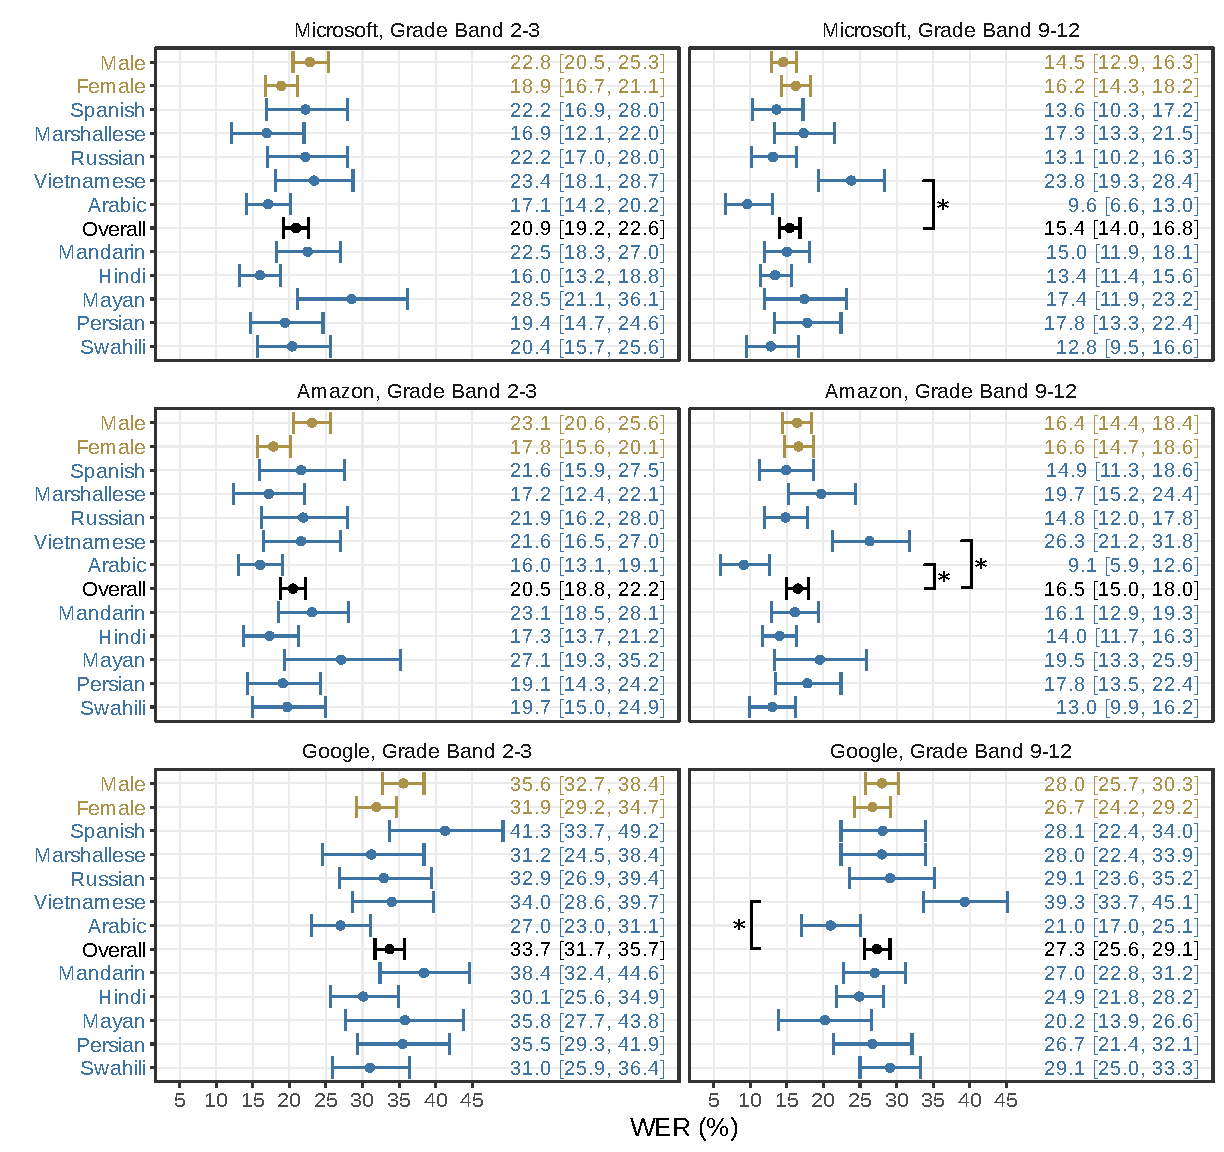
\includegraphics[width=6.5in]{figures/20230513_adj_werPlot_sigBars.pdf}
    \label{fig:wer_all}
{Note: Overall WER appear in black, and disaggregated WER appear in gold (gender) and blue (L1); whiskers indicate 95\% confidence intervals; brackets with asterisks indicate statistically significant pairwise comparisons. \par}
\end{figure}

Automated transcripts were generated from October 7-12, 2022 (for Google and Amazon) and from November 12-13, 2022 (for Microsoft). Transcript requests were sent using Microsoft, Amazon, and Google APIs for Python 3.8.12 \cite{python2022}. Default settings were used for all services. Output language code was set to "en-US" for all three providers. Microsoft required several additional settings: The profanity filter was set to "None", and punctuation mode was set to "Automatic". Microsoft and Amazon provided multiple transcripts by default; in both cases, the most probable transcript was selected for analyses. 

\section{Comparison of WER across datasets}
\label{sec:appendix_l2}

L2-ARCTIC is a publicly available L2 English speech corpus \cite{zhao2018l2}. Similar to the subsample of ELPA21, subjects in L2-ARCTIC were sampled so as to be balanced in terms of gender and L1. Descriptive statistics of the L2-ARCTIC, alongside ELPA21, are presented in Table \ref{tab:l2}. L2-ARCTIC includes a total of 27.1 hours of speech from 24 adults across 6 different L1 (Table \ref{tab:l2}). L2-ARCTIC is comprised of scripted speech: Speakers were asked to read the ARCTIC prompts, a selection of out-of-copyright text curated to be phonetically balanced \cite{kominek2003}. 

\begin{table*}
  \caption{Descriptive statistics of ELPA21 and L2-ARCTIC datasets, with means and standard deviations (in parentheses), overall and disaggregated by gender and L1}
  \small
  \label{tab:l2}
  \centering
  \begin{tabular}{lcccccccc}
  \toprule
    & \multicolumn{4}{c}{\textbf{ELPA21}} & \multicolumn{1}{c}{ } & \multicolumn{3}{c}{\textbf{L2-ARCTIC}} \\
    \cline{2-5}
    \cline{7-9}
    % & \textbf{n} & \textbf{Word count} & \textbf{Duration (sec.)} & \textbf{English proficiency} &  & \textbf{n} & \textbf{Word count} & \textbf{Duration (sec.)} \\ 
    & \multicolumn{1}{p{1cm}}{\centering \textbf{} \\ \textbf{n}} & \multicolumn{1}{p{1.1cm}}{\centering \textbf{Avg.} \\ \textbf{Words}} & \multicolumn{1}{p{1.1cm}}{\centering \textbf{Avg.} \\ \textbf{Seconds}} & \multicolumn{1}{p{1.25cm}}{\centering \textbf{Avg.} \\ \textbf{Proficiency}} &  & \multicolumn{1}{p{1cm}}{\centering \textbf{} \\ \textbf{n}} & \multicolumn{1}{p{1.1cm}}{\centering \textbf{Avg.} \\ \textbf{Words}} & \multicolumn{1}{p{1.1cm}}{\centering \textbf{Avg.} \\ \textbf{Seconds}} \\
    \midrule
\textbf{All} & 1000 & 34 (27) & 24 (15) & 0.04 (1.09) & & 24 & 9940 (356) & 4061 (518) \\
\textbf{L1} &  &  &  &  & &  &  &  \\
\hspace{3mm} Vietnamese & 100 & 35 (24) & 26 (16) & 0.15 (0.97) & & 4 & 10052 (1) & 4320 (280) \\
\hspace{3mm} Mayan & 100 & 19 (17) & 18 (12) & -1.10 (1.13) & & -- & -- & -- \\
\hspace{3mm} Mandarin & 100 & 42 (35) & 29 (21) & 0.63 (0.97) & & 4 & 10038 (13) & 4309 (322) \\
\hspace{3mm} Persian & 100 & 43 (25) & 27 (13) & 0.64 (0.83) & & -- & -- & -- \\
\hspace{3mm} Spanish & 100 & 32 (24) & 23 (12) & 0.01 (1.03) & & 4 & 9767 (557) & 4221 (649) \\
\hspace{3mm} Russian & 100 & 35 (22) & 24 (13) & 0.28 (0.90) & & -- & -- & -- \\
\hspace{3mm} Marshallese & 100 & 29 (25) & 22 (18) & -0.24 (0.90) & & -- & -- & -- \\
\hspace{3mm} Swahili & 100 & 40 (35) & 28 (19) & 0.16 (0.94) & & -- & -- & -- \\
\hspace{3mm} Korean & -- & -- & -- & -- & & 4 & 10049 (4) & 4092 (502) \\
\hspace{3mm} Hindi & 100 & 34 (22) & 24 (13) & -0.28 (1.10) & & 4 & 10046 (4) & 3477 (334) \\
\hspace{3mm} Arabic & 100 & 34 (22) & 23 (11) & 0.10 (0.98) & & 4 & 9689 (692) & 3947 (641) \\
\textbf{Gender} &  &  &  &  & &  &  &  \\
\hspace{3mm} Male & 500 & 32 (25) & 23 (14) & -0.03 (1.07) & & 12 & 9950 (321) & 4178 (410) \\
\hspace{3mm} Female & 500 & 37 (28) & 26 (17) & 0.11 (1.10) & & 12 & 9930 (403) & 3944 (603) \\
\bottomrule
  \end{tabular}
\end{table*}

In the English speech assessment data (ELPA21), across all three services (Microsoft, Amazon, Google), native Vietnamese speakers had a higher WER, on average, compared to other L1s (Figure \ref{fig:wer_l2}. In contrast, native Arabic speakers had a lower WER compared to other L1s. Hindi speakers also had a lower WER; however, this finding was statistically significant only for transcripts generated by Microsoft. 

\begin{figure}[h]
    \centering
    \caption{Average WER estimates produced by Microsoft, Amazon, and Google automated transcription services.}
    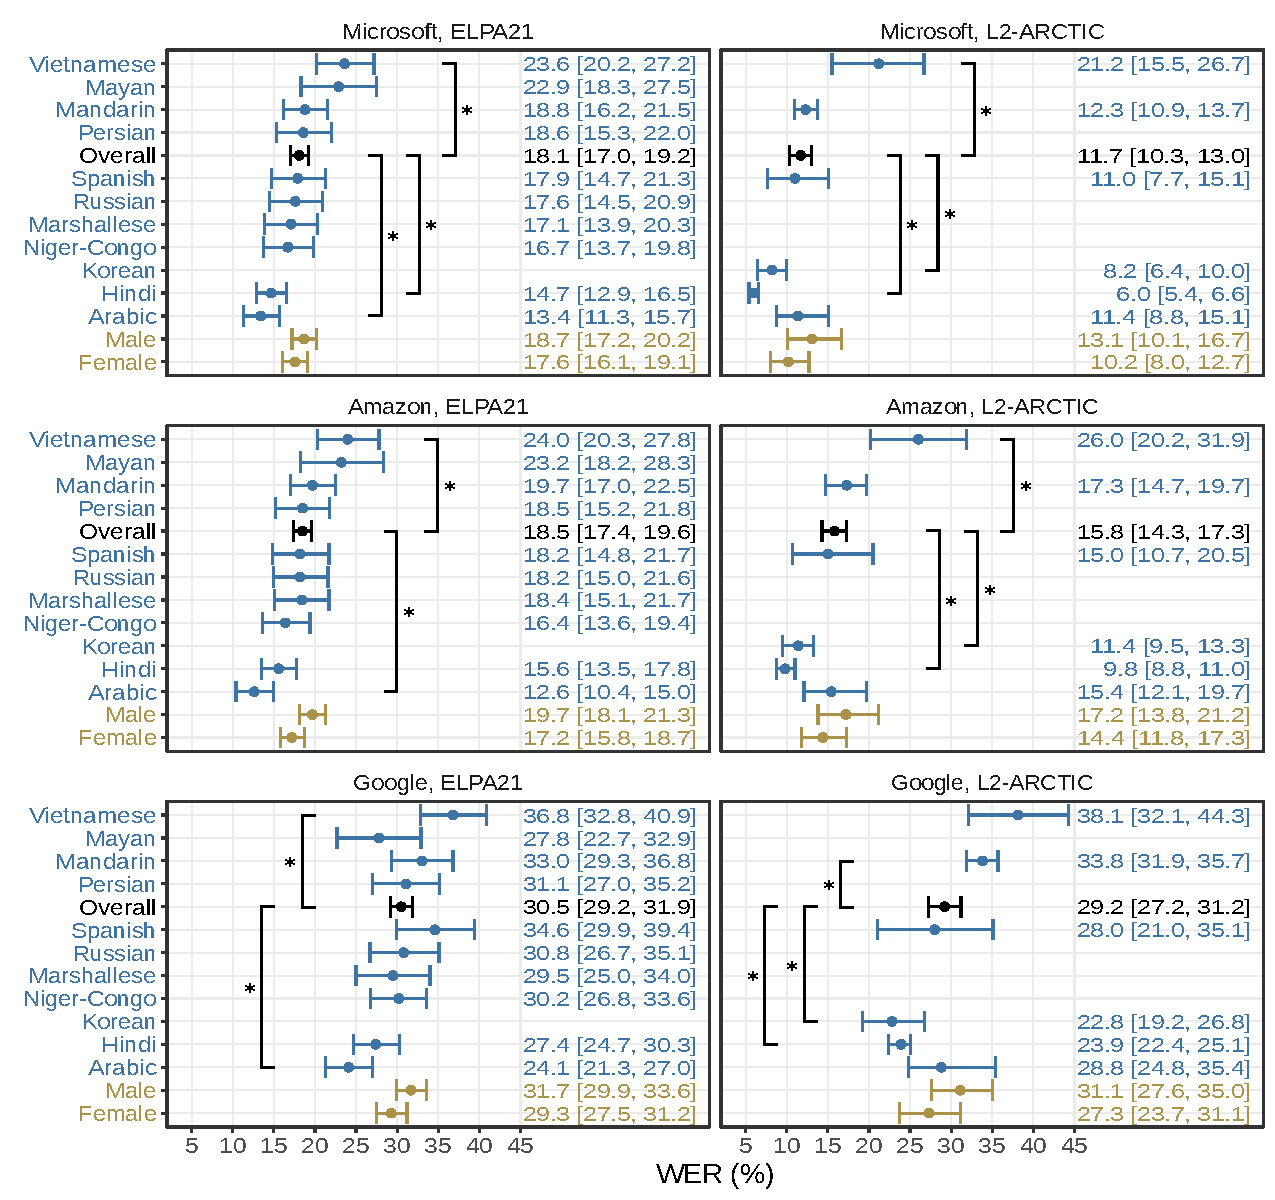
\includegraphics[width=6.5in]{figures/20230308_wer_plot_cmb_sigBars.pdf}
    \label{fig:wer_l2}
{Note: Overall WER appear in black, and disaggregated WER appear in gold (gender) and blue (L1); whiskers indicate 95\% confidence intervals; brackets with asterisks indicate statistically significant pairwise comparisons. \par}
\end{figure}

Some L1 biases were consistent with findings from L2-ARCTIC data. In particular, Vietnamese speakers still had a higher WER, on average, in L2-ARCTIC data--at least for transcripts generated by Microsoft and Amazon. Native Hindi speakers, too, were found to have lower WERs, on average, across all three services in the L2-ARCTIC data. Although neither of these comparisons was found to be statistically in all 6 cases, we consider these findings to be quite robust. 

We were not able to corroborate the finding that native Arabic speakers had a lower WER. In L2-ARCTIC data, native Arabic speakers were not found to have a lower WER than other L1s, on average. 

\section{Human vs. BERT DIF for each item}
\label{sec:appendix_z_itm}

Figure \ref{fig:z_itm} presents the magnitude and direction of DIF of Items 1-3 for grade-bands 2-3 and 9-12, based on gender and all nine L1 focal groups separately.

\begin{figure*}[t]
    \centering
    \caption{Estimates of direction and magnitude of DIF for each of the three speaking items.}
    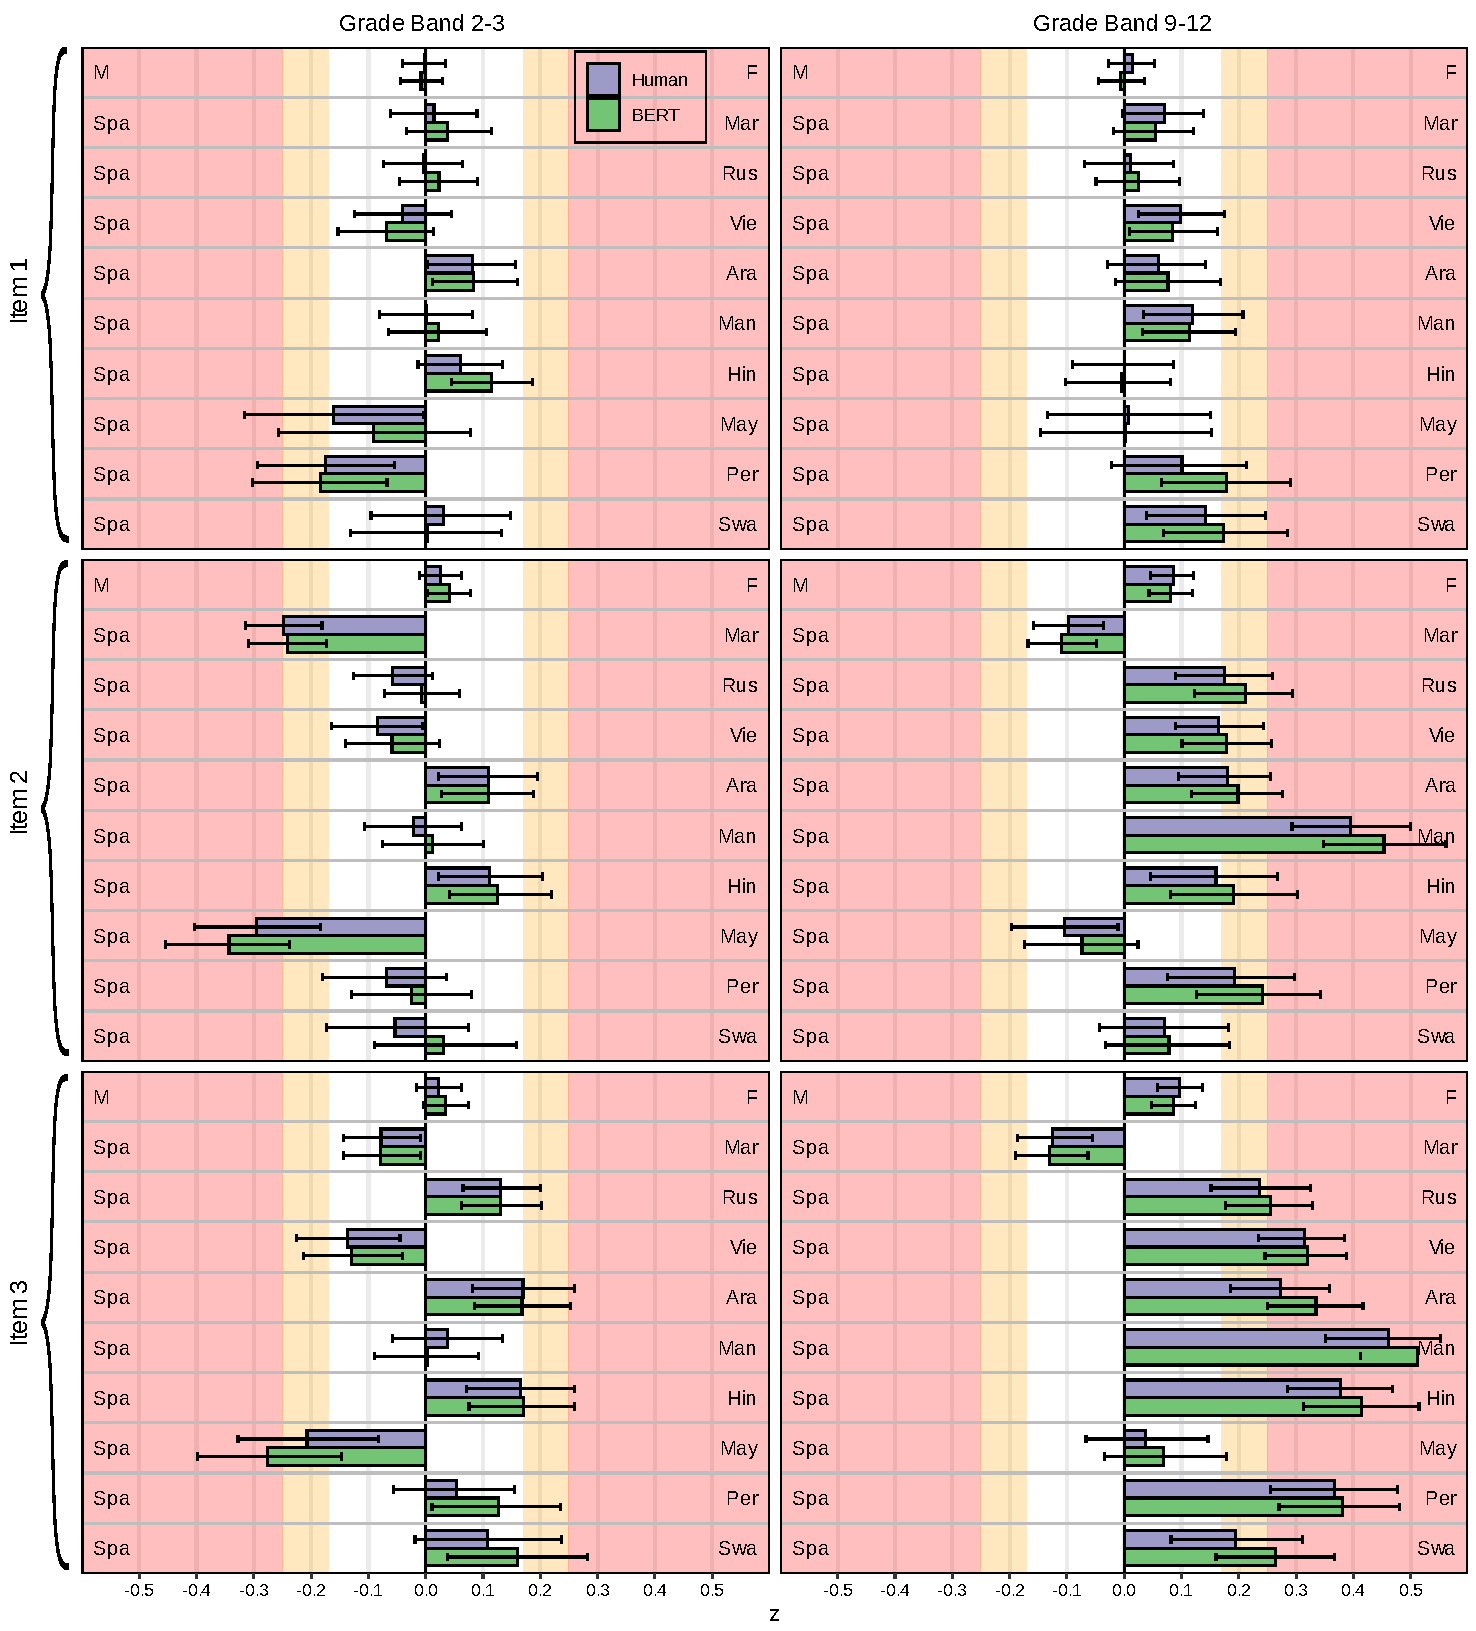
\includegraphics[width=16cm]{figures/20230504_ETS-DIF_BERT_z_itm_edit.pdf}
    \label{fig:z_itm}
{\newline Note: Error bars indicate 95\% confidence intervals. Yellow shaded regions correspond to moderate DIF, and red shaded regions correspond to strong DIF. Reference groups are listed on the left of each chart (M = Male, Spa = Spanish); focal groups are listed on the right (L1 groups are abbreviated by the first three letters). DIF in the positive direction indicates that the focal group is favored. \par}
\end{figure*}

%\bibliography {bib/network,bib/naming}    % bibliography references
\bibliography{20230507_dissertation}
%\bibliographystyle {thesis}
%\bibliographystyle{apa-like}
%\bibliographystyle {uclathes}
%\bibliographystyle{apalike}
%\bibliographystyle{acl_natbib}
\bibliographystyle{plainnat}

\end {document}

